% :autocmd BufWritePost * !pdflatex thesis.tex
\documentclass[a4paper,11pt]{kth-mag}
\usepackage[T1]{fontenc}
\usepackage{textcomp}
\usepackage{lmodern}
\usepackage[utf8]{inputenc}
\usepackage[swedish,english]{babel}
\usepackage{modifications}
\usepackage{amsmath}
\usepackage{amsfonts}
\usepackage{amssymb}
\usepackage{paralist}
\usepackage{listings}
\usepackage{alltt}
\usepackage{subfigure}
\usepackage{draftwatermark}
%\usepackage[firstpage]{draftwatermark}

\SetWatermarkLightness{0.9}
\SetWatermarkScale{1.1}

\usepackage{tikz}
\usetikzlibrary{automata,positioning,shapes.symbols}

% prevent latex from splitting footnotes over multiple pages
% http://www.tex.ac.uk/cgi-bin/texfaq2html?label=splitfoot
\interfootnotelinepenalty=10000


\newcommand{\todo}[1]{\textbf{todo: #1}}
\newcommand{\rephrase}{\textbf{(rephrase)} }

\title{Test-inspired runtime verification}

\subtitle{Using a unit test-like specification syntax for runtime verification}

\foreigntitle{Test-inspirerad runtime-verifiering}

\author{Adam Renberg}
\date{May 2012}
\blurb{Master's Thesis at CSC\\Supervisor Valtech: Erland Ranvinge\\Supervisor
CSC: Dr.\ Narges Khakpour\\Examiner: Prof. Johan Håstad}
\trita{TRITA xxx yyyy-nn}

\begin{document}

\lstset{basicstyle=\ttfamily,
	keywordstyle=\bfseries,
	commentstyle=\color{gray},
	columns=fixed,
	tabsize=2,
	showspaces=false,
	showstringspaces=false,
	numbersep=20pt}

% taken from/inspired by
% http://lenaherrmann.net/2010/05/20/javascript-syntax-highlighting-in-the-latex-listings-package
\lstdefinelanguage{JavaScript}{
  keywords={typeof, new, true, false, catch, function, return, null, catch,
  switch, var, if, in, while, do, else, case, break},
  ndkeywords={class, export, boolean, throw, implements, import, this},
  ndkeywordstyle=\color{darkgray}\bfseries,
  identifierstyle=\color{black},
  sensitive=false,
  comment=[l]{//},
  morecomment=[s]{/*}{*/},
  morestring=[b]',
  morestring=[b]"
}

\frontmatter
\pagestyle{empty}
\removepagenumbers
\maketitle
\selectlanguage{english}




%================================================
%====== The Abstracts
%================================================

\begin{abstract}

% introduction & problem
Computer software is growing ever more complex, and more sophisticated tools
are required to make sure the software operates in a correct way --- i.e.\
according to its specification. Traditional approaches to program verification
have much to give, but they also have their disadvantages. While formal methods
can give nice mathematical proofs about the correctness of programs, they
suffer from complexity and are difficult to use. Often they work only on a
constructed system model, not the actual program. Testing, on the other hand,
has a simple syntax and great tool support, and it is in widespread use. But it
is informal and incomplete, only testing the specific test cases that the
test-writers can come up with.

A relatively new approach called \textit{runtime verification} is an attempt
for a lightweight alternative. It verifies a program's actual
\textit{execution} against its specification, possibly while the program is
running.

% abstract solution
This work investigates how testing, and specifically unit testing, can be
combined with runtime verification. It shows how the syntax of unit tests,
written in the target program's programming language, can be used to inspire
the syntax for specifications for runtime verification. Both informal and
formal specifications are described and supported.

% deliverables
A proof-of-concept framework for Python called \textit{pythonrv} is implemented
and described, and it is tested on a real-life application. A formal foundation
is constructed for specifications written in a subset of Python, enabling
formal verification. Informal specifications are also supported, with the full
power of Python as specification language.

% results & conclusions
The result shows that the proof-of-concept framework allow for effective use of
runtime verification. It is easy to integrate into existing programs, and the
informal specification syntax is quite simple. Many interesting properties can
be verified using it that ordinary tests would have trouble with.

It also shows that formal specifications can be written in Python, but in a
more unwieldy syntax and structure.

% potential
The recommendation for future work lies in improving the specification syntax,
using unit testing concepts such as expectations, and on working to make the
formal specification syntax more like that of its informal sibling.

\end{abstract}
\clearpage


\begin{foreignabstract}{swedish}

Mjukvara växer sig allt mer komplexa, och mer sofistikerade verktyg
krävs för att säkerställa att programmen fungerar korrekt --- at den opererar
enligt sin specifikation. Traditionella tillvägagångssätt till
programverifiering har mycket att ge, men de har också sina nackdelar. Medan
formella metoder kan ge trevliga matematiska bevis om korrektheten av program,
lider de av komplexitet och är svåra att använda. Ofta opererar de bara på en
konstruerad systemmodell, inte det faktiska programmet. Testning, å andra
sidan, har en enkel syntax och bra verktygsstöd, och är i utbredd användning.
Men det är informellt och ofullständigt, testar bara de specifika testfall som
testkrivarna kan komma på.

En relativt ny metod kallad runtime-verifiering är ett försök för ett
lättviktigt alternativ som verifierar ett programs faktiska \textit{exekvering}
mot dess specifikation, eventuellt medan programmet kör.

Det här arbetet undersöker hur testning, och specifikt enhetstestning, kan
kombineras med runtime-verifiering. Det visar hur syntaxen för enhetstester,
skrivna i programmets programmeringsspråk, kan användas som inspiration för
specifikationer för runtime-verifiering.

En proof-of-concept-implementation för Python kallad \textit{pythonrv}
implementeras och beskrivs, och testas på en verklig applikation. En formell
grund framställs för specifikationer skrivna i en delmängd av Python, vilket
möjliggör formell verifiering. Informella specifikationer stöds också, med hela
kraften av Python som specifikationsspråk.

Resultaten visar att proof-of-concept-implemenationen tillåter för effektiv
användning av runtime-verifiering. Den är enkel att integrera i existerande
program, och den informella specifikationssyntaxen är hyfsat enkel. Många
intressanta egenskaper kan verifieras med den som vanliga tester skulle ha
problem med.

De visar också att formella specifikationer kan skrivas i Python, men i en mer
omständigt syntax och struktur.

Rekommendationen för framtida arbete är att förbättra specifikationssyntaxen,
genom att använda koncept från enhetstestning såsom förväntningar, och genom
att göra den formella specifikationssyntaxen mer som den av sin informella
kusin.

\end{foreignabstract}
\clearpage




%================================================
%====== The Preface and ToC
%================================================

\pagestyle{newchap}
\chapter*{Preface}

This is a degree project in Computer Science at the Royal Institute of
Technology (KTH), Stockholm. The work was done at Valtech Sweden, an IT
consultancy.

I've been fortunate to have had two great supervisors: Erland Ranvinge at
Valtech and Dr.\ Narges Khakpour at the School of Computer Science and
Communication, KTH\@. They have been of great help, both in the conception of the
initial idea, and during the project, discussing problems and giving feedback
on the work and this report. Thank you!

I'd also like to thank Valtech for the opportunity to do this degree project as
part of a trainee program, and for all the great colleagues there giving their
feedback and support, especially on the development of the internal web
application described in Chapter~\ref{chapter-evaluation}.

And last, I'd like to thank the many proofreaders. Without them, this report
would be a lot worse. Any errors still in the report are mine and mine
alone.\footnote{For an interesting take on this last sentence, see \emph{The
Preface Paradox} \cite{makinson65prefaceparadox,
williams87prefaceparadoxdissolved}.}

\clearpage

\pagestyle{newchap}
\tableofcontents*
\mainmatter




%================================================
%====== Chapter 1, Introduction
%================================================

\pagestyle{newchap}
\chapter{Introduction} \label{chapter-introduction}

Due to the increasing size and complexity of computer software it has become
increasingly difficult, if not impossible, to assure oneself that the software
works as desired. This is where verification can be helpful. Of the various
approaches used for verification, \textit{testing}, in all its forms, is the
one familiar to most developers, and in it is widespread use. The introduction
of agile development practices and test-driven development has also popularized
the concept of \textit{unit testing}, a form of testing in which small modules
of a program or system are tested individually.

While testing is popular and often works well, it is incomplete and informal,
and thus yields no proof that the program does what it should --- i.e.\ follows
its specification. Formal verification techniques, such as theorem proving and
\textit{model checking} (and its bounded variant), can give such proofs.
However, they suffer from complexity problems (such as \textit{incompleteness},
\textit{undecidability}) and practical issues, such as the so-called
\textit{state explosion} problem.

A relatively new approach in this area is \textit{runtime verification}, in
which the program \textit{execution} is verified against its specification, at
runtime. With the specification written in a suitably formal language, the
execution can be given a mathematical proof that it follows the program's
specification.

This is where this report takes off, with formal verification on one side and
testing on the other, and with runtime verification somewhere in between. Could
the syntax and tooling of unit testing be used to improve the ease of using
runtime verification?


\section{Problem Statement} \label{section-problem-statement}

How can runtime verification specifications be written in a manner that uses
the syntax of the target program's programming language, and resembles the
structure of unit tests? Can we still give a formal semantics to the
specification language, or a part of it? How can we bridge the spectrum of
different approaches for verification, creating something in between the formal
and informal techniques?


\section{Motivation}

Checking that a program works correctly is of great interest to software
developers. Formal verification techniques are helpful, but as mentioned above,
traditional methods can be impractical with larger programs, and verification
by testing is informal and incomplete. Runtime verification can here be a
lightweight addition to the toolbox of verification techniques.

The specification languages used by runtime verification approaches are often
based on formal languages/formalisms (e.g.\ logic or algebra) and not written
in the target program's programming language. This means that writing the
specifications requires specific knowledge and expertise in mathematics. It
also requires mental context-switching, between writing the program and writing
the specification, and special tools to support this specialised language's
syntax.

In contrast, unit testing frameworks often utilise the programming language to
great effect, and they are a common part of the software development process.

However, formal specifications allow for mathematical reasoning and proofs
about properties of the program. A combination of the simpleness of the syntax
and tool-support for testing with the mathematical properties of formal
specifications could add more certainty to the verification in software
development.

If runtime verification specifications more resembled unit tests, and were
written in the target program's programming language, it might popularise the
use of runtime verification for checking the correctness of programs.


\section{Structure of this Report}

The rest of this report is structured as follows. This chapter gives an
introduction to the report and the problem statement.
Chapter~\ref{chapter-background} gives a background to the subject of verifying
program correctness and an overview of formal methods, testing and runtime
verification. Chapter~\ref{chapter-intro-to-rv} continues by describing the
previous research on runtime verification, the syntax of specification
languages and different approaches to code instrumentation.
Chapter~\ref{chapter-intro-to-unit-testing} gives an overview of the current
ideas in unit testing.

Chapter~\ref{chapter-approach} describes the approach this work takes to
solving the problem stated in Section~\ref{section-problem-statement}. It
describes the syntax, instrumentation and verification techniques used in a
proof-of-concept implementation, and gives a formal foundation to a subset of
the syntax. Chapter~\ref{chapter-evaluation} then gives an evaluation of
applying this work on a real-life web application.

Conclusions and a discussion of this and future work is done in
Chapter~\ref{chapter-conclusions}.

The first time an important concept is introduced it is written in
\textit{italics}. If such a concept is not explained in the text, it has a
brief description in the Glossary, see Appendix~\ref{appendix-glossary}.

\section{Limitations}

Naturally, there are some areas that this report does not attempt to solve. The
report describes a proof-of-concept implementation of a runtime verification
framework for Python, with specifications written as Python code. It discusses
both formal and informal specifications, and shows how verification can be done
for both. It does not attempt to formalize Python. It gives a formalization for
only a subset of Python --- for specifications constructed in a special way.

Also, it only deals with a single thread of execution --- no multi-threading or
multiple processes. To limit the scope of the framework, it doesn't directly
expose real-time data to the specifications.

No performance testing or benchmarking is done on the implementation.




%================================================
%====== Chapter 2, Background
%================================================

\pagestyle{newchap}
\chapter{Background} \label{chapter-background}

Runtime verification is a new area of research, but the research on other forms
of verification, such as formal methods and testing, goes back several decades.
The terms used in this area are used slightly differently by different
researchers, so this chapter starts by giving definitions for some concepts
used in this report. Then we give a short overview of the research areas
related to the subject of this report. Section~\ref{section-formal-methods}
explains what is meant by proving the correctness of programs, and
Section~\ref{section-testing} explains what testing is. And finally,
Section~\ref{section-rv} describes runtime verification and its place in the
set of verification approaches.


\section{Terms and Definitions}
\label{section-background-definitions}
\label{section-definition-verification}
\label{section-system-model}

\textit{Verification} is the very broad concept of checking that a program does
what it is supposed to, which can be expressed as "Are we building the program
correctly?". This can be contrasted with \textit{validation}, in which we ask:
"Are we building the correct program?" \cite{boehm81engineeringeconomics}.
Validation is concerned with whether the specifications really capture the
requirements we want for the system. Verification is concerned with assuring
us that the program follows its specification, and it is verification in which
this report takes an interest. Verification includes everything from manually
running the program and parsing through the output, to automated testing
setups, to formal methods.

Both formal methods and testing are thus included in the term verification, and
they are both described in this chapter.

An essential concept in verification is that of a \textit{system model}. A
system model is a construct that represents and describes the behaviour of a
system. It is usually an abstraction of the real system, leaving out the
details that are of no interest to the task at hand, and making other modeling
aspects more prominent.

We use system models constantly in everyday life when we abstract away the
details of how things actually work to a more easy-to-grasp model of how it
seems to work --- e.g., when driving a car, operating a computer, etc. We often
get into trouble when the system model becomes too much simplified, or when it
conflicts with the actual system, because we lose lots of information. A too
detailed system model can give rise to complexity and noise, however, so a
compromise is desirable.

In formal methods, a system model is a mathematical representation of the
system that captures and describes its relevant parts --- the parts of the
system we wish to prove properties about, and reason with formally. In unit
testing, the system model is the unit under test, an isolated slice of the
system, with the rest of the actual system ignored or mocked away.


\section{Formal Methods} \label{section-formal-methods}

Formal methods are verification techniques, based in mathematics, for the
specification and verification of systems. There are several approaches, with
their respective advantages and disadvantages. \textit{Theorem proving} and
\textit{model checking} will be discussed below. They both rely heavily on the
concept of a proof of correctness.

A correctness proof is a certificate, based in mathematics and logics, that a
program/system/function follows its specifications, i.e.\ does what it is
supposed to do.

Research of interest include the early work on formal methods, e.g.\ by Hoare
\cite{hoare69} and Floyd \cite{floyd67}, and work on logics , e.g.\ linear
temporal logic (LTL) by Pnueli \cite{pnueli77}. The seminal work done by Hoare,
Floyd and Pnueli lay the foundation for many interesting approaches. LTL is one
of the common formal languages used for specifications in runtime verification.

\textit{Theorem proving}, as started by Hoare \cite{hoare69}, Floyd
\cite{floyd67} and others, is the manual, semi-automated, or (not so often)
fully automated process of mathematically proving that the system follows its
specification. There are many ways of doing such proofs.

One way is to prove that at all points in the program, given inputs satisfying
some pre-conditions, the outputs will satisfy the post-conditions. By
formulating post-conditions for the exit point(s) of the program so that they
follow the specification, and by linking together the pre-conditions of program
points with their preceding program points' post-conditions, we know that
correct input data will yield correct results.

This way of proving correctness often yields very good results --- a complete
and thorough correctness proof for the program. But it is slow, hard to
automate completely, and therefore requires much manual work.  Wading through
large programs thus often becomes impractical.

\textit{Model checking} is the concept of verifying that a \textit{model} of a
system (the \textit{system model}) follows its specification. This requires
that both the model and the specification is written in a mathematical
formalism. Given this, the task becomes to see if the model satisfies the
logical formula of the specification. It is often simpler than theorem proving,
and can be automated.

The model of the system is usually structured as a finite state machine (FSM),
and verification means visiting all accessible states, checking that they
follow the specification (which also can be represented as an FSM). This can be
problematic, especially when the state space becomes very big, something known
as the \textit{state explosion problem}. There are approaches to address this
issue, such as \textit{bounded model checking}, or by using higher-level
abstractions.

Proving that a model of a system is correct can be very useful, but it suffers
from the inherent flaw of only verifying the model, not the actual system. The
model can be difficult to construct, or deviate too far from the system. It can
not take the dynamic properties and configuration of the executing code into
account.

Runtime verification (Section~\ref{section-rv}) attempts to solve this by
dealing directly with the system, creating its model at runtime.


\section{Testing} \label{section-testing}
Opposite formal methods on the verification spectrum is \emph{testing}, which
is the practical approach of checking that the program, given a certain input,
produces the correct/acceptable output. Testing consists of a set, or
\textit{suite}, of \textit{test cases}. A test case tests some aspect of the
program, from large ("It should be possible to go through the shop flow and buy
a product") to small ("This function should throw an exception when given a
null argument").

Testing can be either manual or \textit{automated}, or something in between. In
manual testing a programmer, tester or other stakeholder, runs the program,
entering some inputs and inspecting the outputs. Test cases could be documents
describing what should happen for given inputs, where to click or type to cause
the desired outcome. In \textit{automated} testing the test cases are
machine-runnable, so that a computer can run them during the development
process, or when checking code into a central repository, or during releases,
etc.

Testing is not complete (for all but the most trivial programs, it is
impossible to write complete tests), and lacks a formal foundation, so it
cannot be used for formal verification. Testing is popular and is used on
virtually all development projects, taking up a large part of development time
(see e.g.\ \cite{brooks75mythicalmanmonth}).

\textit{Unit testing} is the concept of writing tests for small units in a
program, such as functions, classes, etc. These tests are used during
development to test the functionality of the units. The aim is to reduce the
risk of breaking existing functionality when developing new features, or
modifying existing code, by preventing regression. Unit testing is described in
more detail in Chapter~\ref{chapter-intro-to-unit-testing}.



\section{Runtime Verification} \label{section-rv}

Runtime verification (RV) is a dynamic approach to checking program
correctness, in contrast to testing and the more traditional formal static
analysis techniques discussed in Section~\ref{section-formal-methods}.  Runtime
verification aspires to be a light-weight formal verification technique, see
e.g.\ \cite{leucker09abriefaccount,delgado04taxonomy}. It verifies whether
properties of a specification hold \textit{during the execution} of a program.

Runtime verification can be both formal, if the specifications are given a
formal semantics, or informal, if they are more like tests or other program
code.

The specification that should be verified is often written in a formal
language, a logic or a calculus, such as LTL \cite{pnueli77} (this report shows
one exception --- see Chapter~\ref{chapter-approach}). To build a system model
for verifying the properties of the specification, the target program needs to
emit or expose certain events and data. The collected events and data are used
to build the system model. RV frameworks typically use \textit{code
instrumentation} to generate \textit{monitors} for this end.

A monitor is either just part of a recording layer added to the program, which
stores the events and data needed for verification, or also the part of the
machinery that performs verification.

There are two types of verification: \emph{online} and \emph{offline}. In
online verification, the analysis and verification is done during the
execution, in a synchronous manner with the observed system. In offline
verification, a log of events is analysed at a later time. Online verification
allows actions to be taken immediately when violations against the
specifications are detected, but with considerable performance cost. Offline
verification only impacts the performance by collecting data.

When a violation of the specification occurs, simple actions can be taken
(e.g.\ crash the program, log the error, send emails, etc.), or more complex
responses initiated, resulting in a \textit{self-healing} or
\textit{self-adapting} system (see e.g.\ \cite{huebscher08survey}).

Leucker et al.\ present a definition of RV in \cite{leucker09abriefaccount},
together with an exposition of the advantages and disadvantages, similarities
and differences, with other verification approaches. In
\cite{delgado04taxonomy}, Delgado et al.\ classify and review several different
approaches to and frameworks for runtime verification.

The next chapter examines RV in more detail.






%================================================
%====== Chapter 3, Introduction to Runtime Verification
%================================================

\pagestyle{newchap}
\chapter{Introduction to Runtime Verification} \label{chapter-intro-to-rv}

As we saw in Section~\ref{section-rv}, runtime verification is a technique for
verifying a program's compliance against a specification during runtime. These
specifications need to be written somehow, which will be discussed in
Section~\ref{section-specifications}. Approaches for verification are discussed
in Section~\ref{section-verification}. For verification to work, during
runtime, the program usually needs to be instrumented in such a way that the
verification process can access all pertinent data. This is discussed in
Section~\ref{section-instrumentation}


\section{Specifications} \label{section-specifications}

A specification is essentially something that describes the correct behaviour
of a system. Specifications come in many forms, from the informal ones like ``I
want it have cool buttons'', to the contractual ones written between companies
and their clients, to tests (see e.g.\
Chapter~\ref{chapter-intro-to-unit-testing}), and to formal specifications,
written in formal languages, specifying properties that should verifiably hold
for the program (see e.g.\ Section~\ref{section-ltl}). It is these last two
types of specifications that we are interested in here, and which play an
important role in runtime verification.

In general, specifications should be abstract, written in a high-level
language, and succinctly capture the desired property. Writing erroneous
specifications is of course a possibility; specifications need to be easier for
humans to verify than the program's implementation. There is little point in
having a specification as complex as the program itself, except for as a point
of reference. A program can be seen as an all-encompassing, perfect,
always-true, specification of itself.

\section{Related Work}

Temporal Rover, EAGLE, MAC Logic

\subsection{Formalisms for Specifications}

There are several common formalisms for writing specifications, and many papers
that expand, rephrase and illuminate on them. Although they can be quite
different, they share a common origin in the work done by Floyd \cite{floyd67},
Hoare \cite{hoare69}, and others before them. Floyd wrote of formulas as
specifying in/out properties of statements, and chaining these together to form
a formal proof for the program. Hoare elaborated on this idea by basing his
proofs on a few axioms of the programming language and target computer
architecture, and building the proof from there.


\subsubsection{Linear Temporal Logic} \label{section-ltl}

Linear temporal logic (LTL) was first discussed by Pnueli \cite{pnueli77}, and
has since been popular in many areas dealing with a system model containing a
temporal dimension. LTL is simpler than other logics, but expressive enough to
describe many problems of interest for verification. This has been affirmed by
the diverse use of LTL by many researchers \cite{pnueli77}.

LTL uses a system model of \textit{infinite execution traces}, or
\textit{histories}, of the states of the execution. LTL specifications are
formulas that operate on these states. An LTL formula consists of
\textit{propositional variables} that work on the domain model of the state
(checking variables, inputs, global state, etc.), the normal logical operators
such as negation and disjunction, and some temporal operators. The most basic
and common temporal operators are $\boldsymbol{X}$ (\textit{next}), and
$\boldsymbol{U}$ (\textit{until}). Other operators can be derived from these,
such as $\boldsymbol{G}$ (\textit{globally}, or always) and $\boldsymbol{F}$
(\textit{eventually}, or sometime in the future).

An example LTL formula, taken from a list of common specification patterns
\cite{dwyer99patterns}, could be: $S$ precedes $P$, i.e.\ if the state $P$
holds sometime, the state $S$ will hold before it. This is shown in
Figure~\ref{figure-ltl}.

\begin{figure}[h!]
	\[
	\boldsymbol{G} \, P \rightarrow (\neg P \, \boldsymbol{U} \, (S \wedge \neg P)
	\]

	\caption{An example of an LTL formula. This can be read as: Globally, if $P$
	holds, then, before $P$, $S$ held at some point.}
	\label{figure-ltl}
\end{figure}

Bauer et al.\ \cite{bauer06monitoring} introduce a three-valued boolean
semantics for LTL, calling it LTL$_3$, which takes the values (true, false
and~?). This logic is arguably more suited for the finite nature of runtime
verification, whereas LTL was designed with infinite traces in mind. The
semantics of LTL$_3$ reflect the fact that when verifying runtime verification
specifications, the result can not only be that the specification is satisfied
or violated; it can be inconclusive as well. For satisfied or violated
specifications, no further verification is required --- we already know the
outcome. For inconclusive results, we need to continue with the verification,
as, with future events, the result could change into either satisfied or
violated.

There is a counterpart to LTL in the real-time setting called Timed Linear
Temporal Logic (TLTL). It introduces clocks to make specifications
of real-time properties possible. It is of great interest to runtime
verification, but will not be discussed further here. See e.g.\
\cite{bauer06monitoring} for more.

\subsubsection{EAGLE and RuleR}

Barringer et al.\ have written EAGLE \cite{barringer03eagle} and RuleR
\cite{barringer07ruler} as runtime verification frameworks and formal logics.
Inefficiency weaknesses were found in EAGLE, and RuleR was proposed as a more
efficient alternative, with a more lower-level logic. They share much of the
same basic ideas, however --- they are written by mostly the same people.

EAGLE can be seen as a generalization of other logics, supporting both past and
future tense predicates. It is a temporal finite trace monitoring rule-based
logic, meaning that a specification consists of a set of rules, which operate
on finite sequences of states of the system model, each state being part of a
program execution.

A simple example of an EAGLE formula is shown in
Figure~\ref{figure-eagle-always}.
It describes the LTL operator $\boldsymbol{G}$. $\bigcirc$ is the same as the
LTL \textit{next} operator $X$, and \textbf{Form} is the type of $F$, short for
formula. The \textbf{max} qualifier denotes that a maximal solution should be
found for the equation. $\bigcirc \text{Always}(F)$ is thus defined to be true
in the last state of a given trace. A corresponding \textbf{min} qualifier also
exist.

\begin{figure}[h!]
	\[
  \textbf{max} \; \text{Always}(\textbf{Form} \; F) = F \wedge \bigcirc \text{Always}(F)
	\]

	\caption{A simple example of an EAGLE formula, semantically describing the
  LTL $\boldsymbol{G}$ operator. Taken from \cite{barringer03eagle}.}
	\label{figure-eagle-always}
\end{figure}

The same property can be described in RuleR. If we let $\{r\}$ be the initial
set of rule activations, the formula in Figure~\ref{figure-ruler-always} say
that rule $r$ requires an observation of $r$ in this state, and that the rule
$r$ should hold in the next state.

\begin{figure}[h!]
	\[
    r \; : \; \rightarrow \; a,r
	\]

	\caption{A simple example of a RuleR formula, semantically describing the
  LTL $\boldsymbol{G}$ operator. Taken from \cite{barringer07ruler}.}
	\label{figure-ruler-always}
\end{figure}

An EAGLE formula describing the LTL formula from Figure~\ref{figure-ltl} is
shown in Figure~\ref{figure-eagle-ltl}. Note the use of the \textbf{min} and
\textbf{max} quantifiers. Here they mean that PreviouslySometime$(F)$ should be
defined as false on the first state, while PreviouslyAlways$(F)$ should be
true.


\begin{figure}[h!]
  \[
  \begin{array}{rcl}
    \textbf{min} \; \text{PreviouslySometime}(\textbf{Form} \; F) & = & F \vee \odot \, \text{PreviouslySometime}(F) \\
      \textbf{max} \; \text{PreviouslyAlways}(\textbf{Form} \; F) & = & F \wedge \odot \, \text{PreviouslyAlways}(F) \\
  \end{array}
  \]
  \[
    \text{Always}(P \rightarrow (\text{PreviouslySometime}(S) \wedge \text{PreviouslyAlways}(\neg P) \\
  \]

	\caption{A simple example of an EAGLE formula, semantically the same as the
  LTL formula from Figure~\ref{figure-ltl}.}
	\label{figure-eagle-ltl}
\end{figure}

Both EAGLE and RuleR are strictly more powerful than LTL; e.g., they both
support specifications that allow matching function calls with function
returns, the realm of context-free grammars. LTL does not support this
\cite{barringer03eagle,barringer07ruler}.

\subsubsection{Temporal Rover}

\todo{A short description of Temporal Rover's Logic}


\subsubsection{Design by Contract}

\textit{Design by Contract} is a verification technique similar to runtime
verification, without the ability to describe temporal properties. Design by
Contract was introduced by Bertrand Meyer in \cite{meyer92applyingdbc}, and has
been fully implemented in the Eiffel programming language\footnote{See
\texttt{http://eiffel.com/} and
\texttt{http://se.ethz.ch/~meyer/publications/online/eiffel/basic.html} for a
description of the language.}. An example can be seen in
Figure~\ref{figure-dbc-example}.

\begin{figure}[h!]
	\begin{center}
	\begin{minipage}{0.7\textwidth}
    \lstset{language=Eiffel}
		\lstinputlisting{figures/dbc_example.e}
	\end{minipage}
	\end{center}
  \caption{An example showing the use of the Design-by-Contract concepts of
    pre- and post-conditions, written in Eiffel. Note the use of the language
    construct \texttt{old} to get the value of an attribute at before the
    function executed. Example taken from \cite{meyer92applyingdbc}.}
	\label{figure-dbc-example}
\end{figure}

A contract is the idea that functions, and methods on objects, promise to
satisfy certain post-conditions (or promises) if the inputs they are given
satisfy the pre-conditions (or requirements) specified in the contract. Design
by Contract also contains constructs for specifying loop-invariants and
class-invariants, properties that should always hold during loops and for
objects of a class, respectively. Assertions (see below) are also usually
available, to be interspersed with the program code.

Design by Contract is inspired by Hoare logic, and is essentially Hoare logic
written in a certain style. However, most implementation of Design by Contract,
such as that of Eiffel, and Code
Contracts\footnote{\texttt{http://msdn.microsoft.com/en-us/devlabs/dd491992.aspx}}
in~.Net, allow for arbitrary code in the specifications. The specifications are
thus informal, unless a formalization is given for the programming language
used.


\subsubsection{Assertions}

A common construct that is part of many popular programming languages, like C,
Java and Python, is the \textit{\texttt{assert} statement}. It is a way to
state that some predicate should hold at a point in the program. Usually the
predicate is an expression in the programming language, and is not supposed to
alter the program state. See Figure~\ref{figure-c-assert-example} for an
example.

\begin{figure}[h!]
	\begin{center}
	\begin{minipage}{0.7\textwidth}
    \lstset{language=C}
		\lstinputlisting{figures/cassert_example.c}
	\end{minipage}
	\end{center}
  \caption{An example showing the use of \texttt{assert} in C. Note that the
    return value of \texttt{malloc} is checked to be non-null using an
    if-statement --- this is a case that could happen. The assertions are used
    to check for cases that should never happen.}
	\label{figure-c-assert-example}
\end{figure}

Assertions are distinct from the normal program flow, and not to be conflated
with exceptions. Assertions check for properties that should always be true,
anything else would be a programming error. Assertions can sometimes be turned
of with a compiler or runtime flag.

Assertions are suitable for simpler specifications, and those more coupled to
code. Assertions are the simplest of runtime verification specifications. If
the languages they are part of are informal, the specifications they represent
are informal as well.


\subsection{Developing with Specifications}

For verification in general, specifications can be written and used externally
to the program. They can be used in specialized model-checking tools, in tools
for theorem proving, etc.

Runtime verification requires that the specifications are accessible when
building and running the program. At the very least, the program needs to be
instrumented to expose the correct system model so that the specification can
be verified. It is sometimes desired in runtime verification to do online
verification, and then the specifications need to be available and embedded
into the system. A few different approaches have been tried to support this.

Approaches to writing specifications can be divided into two parts: those that
require you to manually mark code for verification, and those that inject the
verification code from external specifications.

Rosenblum \cite{rosenblum95practicalassertions} uses specially annotated
comments, written directly in the code. Bodden
\cite{bodden05efficientrv,bodden04lightweightltl} uses Java annotations, which
are written at function and variable definitions, to mark code for
verification. The programming language Eiffel has full language support for
Design by Contract, with pre- and post-conditions, invariants, and more. These
are written in direct proximity to the code to be verified. For simple cases it
is common to write assertions in the program \cite{bartetzko01jass}.

Other approaches, such as the ones taken by Jalili et al.\ in
\cite{jalili07rverl} and Barringer et al.\ in \cite{barringer03eagle}, use
external specification files, and the program is instrumented at compile- or
runtime for verification.



\section{Verification against Specifications} \label{section-verification}

Specifications for runtime verification are written so that programs can be
verified against them --- to see whether they follow the specification, or
violate parts of it.

There are several ways to verify a program against its specification. A common
one, used in \cite{bauer06monitoring, bodden05efficientrv, jalili07rverl,
barringer03eagle} among others, is to generate state machines from the
specification. These state machines, sometimes called \textit{runtime
monitors}, operate with the input language of events emitted by the program. As
the program executes, or a program execution is replayed offline, transitions
are taken in the state machines, switching states. Violations against the
specification can be described by failing to find a valid transition, or ending
up in a fail state; Fulfilling a specification can be described by arriving at
an accepting state.

Simpler verification approaches just instrument the code by adding assertions
that check the properties of the specifications. This might be difficult to do
with more complex specifications.


\section{Code Instrumentation} \label{section-instrumentation}

For verification to work, the verifier needs access to events happening in the
program. Such events can be functions called, statements executed, variables
assigned, etc., depending on the system model of the specification language.
The program needs to be instrumented for it to emit such events. This often
means wrapping function calls and variable assignments in a ``recording
layer'', which performs the desired action after logging the event. The events
can then be passed on to the verification tools.

What follows are four major approaches used for program instrumentation.


\subsection{Pre-processing the Code}

Rosenblum \cite{rosenblum95practicalassertions} uses a pre-processor step in
the C compilation setup to instrument code, where the specifications (called
assertions by Rosenblum) are transformed from comments into regular C code. See
Figure~\ref{figure-pre-processing-comments-example} for an example. The
verification code is then compiled together with the program.

\begin{figure}[h!]
	\begin{center}
	\begin{minipage}{0.7\textwidth}
    \lstset{language=C}
		\lstinputlisting{figures/instrumentation_comments_example.c}
	\end{minipage}
	\end{center}
  \caption{An example showing instrumentation via special comments and code
    pre-processing. Example taken from \cite{rosenblum95practicalassertions}.}
	\label{figure-pre-processing-comments-example}
\end{figure}

\subsection{Post-processing the Code}

It is also possible to rewrite the compiled program, instrumenting the code
after compilation. This way, the program needs no knowledge of the verification
framework. Depending on the compiled objects, this can be more or less
difficult. Binary executables and intermediate formats, such as Java bytecode
or Common Intermediate Language for the Common Language Infrastructure used
by~.Net, require somewhat different approaches.


\subsection{Dynamic Code Rewriting}

In many dynamic languages, such as Python, Ruby or JavaScript, it is possible
to rewrite the code during runtime, which is sometimes called \textit{monkey
patching}. A function to be monitored could be rewritten, adding a lightweight
wrapper that records all calls to it, and then passes on the call to the actual
function.


\subsection{Aspects} \label{section-aspects}

An interesting approach to code instrumentation is to use aspect-oriented
programming. In aspect-oriented theory, a program should be divided into
modules, each only dealing with their own \textit{concern}. Logging, however,
is a \textit{crosscutting concern}, as it is used by several unrelated modules.
The goal is to not scatter logging code across the modules, and to not tangle
it with the modules' own logic. This can be done by defining the logging code
as \textit{aspects}, which consists of the logging code, called the
\textit{advice}, and a \textit{point cut}, which is a formula describing when
the advice should be executed. The possible execution points for a point cut
are called \textit{join points}.
AspectJ\footnote{\texttt{http://www.eclipse.org/aspectj/}} is the canonical
framework for aspect-oriented programming.

Runtime verification is a typical case of a cross-cutting concern. Bodden
\cite{bodden05efficientrv} uses AspectJ in his runtime verification
implementation.

Aspects in AspectJ are implemented as a post-processing step in the compilation
process, adding wrapper code for handling the aspects.





%================================================
%====== Chapter 4, Introduction to Unit Testing
%================================================

\pagestyle{newchap}
\chapter{Introduction to Unit Testing} \label{chapter-intro-to-unit-testing}

We discussed testing and in general in Section~\ref{section-testing}. Here
we'll delve into more detail about unit testing in particular, and discuss how
it works, and what the syntax is like.

In unit testing, a program is divided into small, separate parts --- silos,
with minimum dependencies to the rest of the system --- and each unit is tested
in isolation. Dividing a program into these kinds of units can be difficult,
and proponents of unit testing argue that it requires a decoupled and modular
system design.

Unit testing is quite young, perhaps having begun in earnest in the 90s, and it
was popularized by the extreme programming (XP)
movement\footnote{\texttt{http://www.extremeprogramming.org/}}. Testing in
general is very old.

Kent Beck introduced the style of the modern unit testing framework in his work
on a testing framework for Smalltalk \cite{becksmalltalktesting}. Together
with Eric Gamma he later ported it to Java, resulting in
\textit{JUnit}\footnote{\texttt{http://www.junit.org/}}.
Today, this has lead to \textit{frameworks} in several programming languages,
and they are collectively called xUnit \cite{fowlerxunit}. Examples include,
beside JUnit for Java:
\textit{unittest}\footnote{\texttt{http://docs.python.org/library/unittest.html}}
for Python,
\textit{NUnit}\footnote{\texttt{http://www.nunit.org/}} and
\textit{xUnit.net}\footnote{\texttt{http://xunit.codeplex.com/}} for C\#
and~.Net,
\textit{RSpec}\footnote{\texttt{http://rspec.info/}} and the
\textit{Test::Unit}\footnote{\texttt{http://www.ruby-doc.org/stdlib-1.9.3/libdoc/test/unit/rdoc/Test/Unit.html}}
package for Ruby,
and \textit{Jasmine}\footnote{\texttt{http://pivotal.github.com/jasmine/}} for
JavaScript.


When discussing testing, and unit testing in particular, we must mention the
concept of test-driven development (TDD). Also made popular by XP, it consists
of the cycle:
\begin{inparaenum}[1\upshape)]
  \item write a failing test;
  \item make it pass by writing the simplest code you can; and
  \item refactor --- rewrite the code, cleaning it up and giving it a better
    structure.
\end{inparaenum}
Tests here play the part of specifications for the units of the program.


\section{xUnit} \label{section-xunit}

The xUnit style of unit testing \cite{fowlerxunit} has given rise to unit
testing frameworks for many programming languages. Their structure are all
based on the same concept, and since JUnit is the canonical implementation, and
one of the first, implementation, we will use it for a short demonstration. See
Figure~\ref{figure-junit}. Jasmine, being younger and more ``hip'', has a
slightly different syntax, but essentially the same structure. See
Figure~\ref{figure-jasmine}.

\begin{figure}[h!]
	\begin{center}
	\begin{minipage}{0.9\textwidth}
		\lstset{language=Java}
		\lstinputlisting{figures/junit_example.java}
	\end{minipage}
	\end{center}
  \caption{An example of unit testing syntax, written Java as a test case for
    JUnit. All tests are marked with the \texttt{@Test} annotation. The
    \texttt{assert} keyword and functions like \texttt{assertEquals} are used
    to verify the correctness of the outputs.}
	\label{figure-junit}
\end{figure}

\begin{figure}[h!]
	\begin{center}
	\begin{minipage}{0.9\textwidth}
		\lstset{language=JavaScript}
		\lstinputlisting{figures/jasmine_example.js}
	\end{minipage}
	\end{center}
  \caption{An example of unit testing syntax, written in JavaScript and
    Jasmine. It consists of a \texttt{describe} test suite, and one test case
    \texttt{it}, called a specification in jasmine parlance. The
    \texttt{expect(\dots).toEqual(\dots)} style is used for verification.}
	\label{figure-jasmine}
\end{figure}

In JUnit, and xUnit, you run a \textit{test suite} of \textit{test cases},
which contain tests. The example in Figure~\ref{figure-junit}, the test suite
is implicitly created by JUnit, although it is possible to create it and
control it your self. A \textit{test runner} runs the test suite, reporting
progress to the user. When the tests are finished, any errors are displayed.

In the example in Figure~\ref{figure-junit} has two tests, and methods to set
up and tear down the tests \textit{fixture}. These functions are usually called
\textit{setUp} and \textit{tearDown}, respectively, and are called before and
after each test. The fixture is the surrounding set of objects (environment)
that the object under test requires to work properly.

Test written in the style of Figure~\ref{figure-junit} are traditional unit
tests.


\section{Mocking and Faking} \label{section-mocking}

A common issue when writing unit tests is that, to instantiate some object X,
or to call some function Y, the program needs access to some other objects Z. Z
might be something simple, which we can easily create in the test. It might
also be a network or database connection, or something doing heavy calculation,
or just something complex.

One way to work around this is to create fake objects (also called mock-, fake-
or spy objects). A fake network connection has the same interface as a real
network connection, but calling it does not actually transmit anything
anywhere, and it might return pre-defined, hard coded data. Fake objects could
save what actions are taken upon them, and the test could then verify that
these are according to expectations.


\section{Expectations} \label{section-expectations}

Instead of writing fake objects, we can create a mock object and pre-record
what actions we expect to be taken upon them. This is called writing
\textit{expectations} \cite{fowler07expectations}. A simple example of
expectations is shown in Figure~\ref{figure-expectations}.

\begin{figure}[h!]
	\begin{center}
	\begin{minipage}{0.9\textwidth}
		\lstset{language=Java}
		\lstinputlisting{figures/expectations_example.java}
	\end{minipage}
	\end{center}

	\caption{An example of expectations, written using jMock and JUnit.
	Example taken from \cite{fowler07expectations}.}
	\label{figure-expectations}
\end{figure}

Figure~\ref{figure-expectations} shows a test of a fictional shop. The test
tests only one thing, the fill method of the Order object, but it requires a
Warehouse object, for access to the inventory. We supply a mock Warehouse, with
expectations on which methods should be called on it, with which arguments and
what they should return.

An expectation follows a simple pattern:

\begin{itemize}
	\item A function, with an optional object, which is expected to be called.
	\item An invocation count of how often the function is expected to be called.
	\item Expected arguments for the function call. These can be explicit values,
		or generic types, or rules defining the acceptable values.
	\item The return value and modifications to the global state; what should
		happen when the function is called.
	\item When the function call should happen, e.g.\ in what sequence of
		function calls, in what global state.
\end{itemize}

There are two common ways of specifying expectations: recording and explicit
specification. Figure~\ref{figure-expectations} shows an example of how to
explicitly specify expectations.

When recording expectations, you create a mock object and call the expected
functions, with expected arguments and return values, in the expected order.
Then you set the mock into replay mode, and it will replay the recorded
expectations, and verify that they occur correctly.

There are several frameworks for working with expectations, such as
jMock\footnote{\texttt{http://www.jmock.org/}} for Java, Rhino
Mocks\footnote{\texttt{http://ayende.com/wiki/Rhino+Mocks.ashx}} for~.Net and
Ludibrio\footnote{\texttt{https://github.com/nsigustavo/ludibrio/}} for Python.

With both runtime verification and unit testing introduced, a combination of
the two will be the main subject in the next two chapters.





%================================================
%====== Chapter 5, Approach
%================================================

\pagestyle{newchap}
\chapter{Approach} \label{chapter-approach}

With all this background overview and introductions out of the way it is time
for the core and main substance of this report.

\section{Introduction}

As stated in Section~\ref{section-problem-statement}, the objective of this
report is to investigate whether it is possible to do runtime verification with
specifications written in the target program's programming language, structured
similar to unit tests. To find a solution for this, there are four issues we
need to address:

\begin{enumerate}
  \item How should the syntax for the specifications be defined, so that it
    looks similar to that of unit tests, but works for runtime verification?
    Which language should be used? Which unit testing framework to take
    inspiration from?
	\item How should the program be instrumented to monitor the system, to expose
		the appropriate events and data, and to build the system model?
  \item How will this be used to verify the system against the specification?
    Should the verification be done online or offline? Which techniques should
    be used to verify the monitored system against the specification?
	\item How can the resulting approach be provided with a formal foundation?
\end{enumerate}

This report is a documentation on how to solve these issues. The following
sections are each dedicated to one issue, and shows a proof-of-concept of these
ideas. The implementation, called \textit{pythonrv}, can be found
online\footnote{\texttt{https://github.com/tgwizard/pythonrv}}.


\subsection{Definitions}

The following definitions will be used through the next few sections.

\begin{itemize}
  \item A \textit{specification} is a construct that determines the correct
    behaviour of a program. It could be a document, describing the programs
		functionality, or a set of inputs and outputs, describing the correct
		results of the program's computation on that set. It could be a reference
		implementation\footnote{For instance, the only specification for Python is
		the canonical CPython implementation. Python is defined as ``what CPython
		does''.}. A \textit{formal specification} is a mathematical construct that
		can be used in verification proofs to show that a program works correctly,
		i.e.\ according to its specification.

	\item In \textit{pythonrv} a \textit{specification function} is a Python
		function describing a specification, which \textit{pythonrv} can use for
		verification of the program.

  \item A specification function \textit{monitors} points of the program, and
    the points being monitored are called \textit{monitorees}. Currently only
    functions are supported as monitorable points.
\end{itemize}


\subsection{Implementation Language Discussion}

During the development of this proof-of-concept, the biggest factor in deciding
what language to use was how it would assist in instrumentation.
Instrumentation is discussed in Section~\ref{section-approach-instrumentation}.
The language should also be in wide use, support quick development, and have an
active testing culture.

Easy access to a non-trivial and actively used system for real-world testing
would be a plus. More on this in Chapter~\ref{chapter-evaluation}.

Python\footnote{\texttt{http://www.python.org}}, among several languages, fits
these criteria, and was chosen as the implementation language. Python is a
dynamic programming language, commonly running inside a virtual machine.
Perhaps the most striking feature of Python is its use of indentation as block
delimiters. An increase in indentation starts a new block; a decrease marks the
end of the current block.

The name \textit{pythonrv} clearly reflects that it is a framework for runtime
verification in Python.

The syntax, described in the next section, of the \textit{pythonrv}
specifications are naturally heavily influenced by the fact that they are
written in Python.


\section{Syntax} \label{section-approach-syntax}

The canonical framework for doing unit testing in Python is the
\textit{unittest} framework that is included in all modern versions of Python.
Not much development has happened on it in the last years. Many new frameworks
have have spawned, such as PyUnit, Nose and py.test. They build upon the style
of unittest and mostly add new miscellaneous features, such as better test
reporting. The original structure of the unit tests is still prevalent ---
unittest builds on the xUnit style of unit testing, discussed in
Chapter~\ref{chapter-intro-to-unit-testing}.

The next section will illustrate the syntax of \textit{pythonrv}.

\subsection{General Structure of a Specification}

The structure of a informal \textit{pythonrv} specification function is shown
in pseudo-code in Figure~\ref{figure-pseudo-spec}. For the structure of formal
specifications, see Section~\ref{section-approach-formal-foundation}. The next
section illustrates the \textit{pythonrv} syntax for informal specifications
with three concrete examples

\begin{figure}[h!]
	\begin{center}
	\begin{minipage}{0.7\textwidth}
    \begin{alltt}
\emph{import} pythonrv module
\emph{import} modules with functions to be monitored

\emph{annotate} the spec with its monitorees
\textbf{define} specification function \textit{spec}(\textbf{event}):
  taking a special \textbf{event} argument

  with a body of arbitrary Python code
  that verifies that the provided event is correct
  and throws an \textbf{AssertionError} exception when it is not
    \end{alltt}
	\end{minipage}
	\end{center}

  \caption{The structure of a \textit{pythonrv} specification. Note that the
    Python \texttt{assert} statement throws an \texttt{AssertionError}
    exception when its argument evaluates to \texttt{False}.}
	\label{figure-pseudo-spec}
\end{figure}

\subsection{Three Examples of Informal Specification Functions}
\lstset{language=Python,numbers=left}

\begin{figure}[h!]
	\begin{center}
	\begin{minipage}{0.7\textwidth}
	\lstinputlisting{figures/syntax_example_1.py}
	\end{minipage}
	\end{center}

  \caption{A specification that monitors the function \texttt{fib} in the
    module \texttt{fibmodule}. The monitored function is, locally to the
    specification function, aliased as \texttt{func}. The specification asserts
    that the first input to the monitored function is always greater than
    zero.}
	\label{figure-syntax-example-1}
\end{figure}

The example in Figure~\ref{figure-syntax-example-1} shows the basics of a
\textit{pythonrv} specification, written as a specification function. Line 1
imports the \texttt{rv} module from the \texttt{pythonrv} package. On line 2 it
imports the module containing the function to be monitored. Line 5 defines
the specification as an ordinary Python function called \texttt{spec}, taking
one argument, \texttt{event}. The instrumentation is done line 4 by using the
\textit{function decorator}\footnote{See
Section~\ref{section-approach-instrumentation} for an explanation of function
decorators and \texttt{rv.monitor}.} \texttt{rv.monitor}. \texttt{rv.monitor}
declares that the function \texttt{fib} in \texttt{fibmodule} should be
monitored, and, whenever \texttt{fib} is called, \texttt{spec} should be called
as well.

The specification function itself consists of any valid Python code. It is
passed a special argument, \texttt{event}, which gives the specification
function access to data about the current event. On line 6, the array of input
arguments used to call \texttt{fib} is accessed to check that the first
argument is greater than zero.

The specification function in Figure~\ref{figure-syntax-example-1} will be
called upon every invocation to \texttt{fibmodule.fib}.

\begin{figure}[h!]
	\begin{center}
	\begin{minipage}{0.7\textwidth}
	\lstinputlisting{figures/syntax_example_2.py}
	\end{minipage}
	\end{center}

	\caption{A specification that monitors two functions, \texttt{mymodule.foo}
		and \texttt{mymodule.bar}. It asserts that calls to the two functions
		alternate; that no two calls to \texttt{foo} occurs without a call to
		\texttt{bar} in between, and vice versa. The first call has to be to
		\texttt{foo}.}
	\label{figure-syntax-example-2}
\end{figure}

Figure~\ref{figure-syntax-example-2} shows how a specification function can
monitor two functions. The specification function will be called whenever
either of the monitored functions are called. Which function was called can be
determined from the \texttt{event} argument, as is done on lines 7 and 14. It
is the \texttt{called} attribute of a function in the \texttt{event.fn}
structure that allows for this.

The example also shows how the specification can access a history of previous
events - events that it has handled in the past. \texttt{event.history} is a
list of all events that has occurred that this specification monitors. The last
element is the current event, and the next-to-last element is the previous
element, which can also be accessed as \texttt{event.prev}.

\begin{figure}[h!]
	\begin{center}
	\begin{minipage}{0.7\textwidth}
	\lstinputlisting{figures/syntax_example_3.py}
	\end{minipage}
	\end{center}

	\caption{A more complex example: A specification function that monitors three
		functions, \texttt{foo}, \texttt{bar} and \texttt{baz}, and makes sure that
		\texttt{foo} is called first, then any number calls to \texttt{bar} with
		the first argument as \texttt{True}, and then finally a call to
	\texttt{bar}. After that, any calls are allowed --- the specification function
will not be used in verification any longer.}
	\label{figure-syntax-example-3}
\end{figure}

Figure~\ref{figure-syntax-example-3} shows a more advanced example, in which
the \texttt{next} function of the \texttt{event} argument is used.
\texttt{event.next} allows the specification function to add more specification
functions (possibly implemented as closures or lambdas) to be executed when the
next event occurs.

On line 9 the function \texttt{followup} is added to be executed on the next
event. Since \texttt{followup} is added in this way --- as a ``oneshot''
specification function --- it needs to add itself using \texttt{next} for
verification on subsequent events. This is done on line 22.

Figure~\ref{figure-syntax-example-3} also shows how a specification function
can turn its verification off --- i.e.\ unsubscribe from future events.
\texttt{event.finish} and \texttt{event.success} are essentially the same, and
unsubscribes without further errors. \texttt{event.failure} can be thought of
as a combination of \texttt{event.finish} and \texttt{assert False} (which
always fails).


\subsection{Capabilities and Limitations}

The examples above show the main capabilities of \textit{pythonrv}
specifications. A few minor details were left out, such as how to specify how
much history should be saved for a specification, or how to label
specifications with error levels, so that different actions can be taken
depending on which specification function fails. This is described on the website for
\textit{pythonrv}.


\section{Instrumentation} \label{section-approach-instrumentation}

The previous section showed how \textit{pythonrv} specification functions can
be written. This section will describe how these functions can jack themselves
into the ordinary control flow of the program and gain access to the function
call events and their arguments and associated state.

Instrumentation is done through the \texttt{rv.monitor} \textit{function
decorator} in \textit{pythonrv}. A Python function decorator is similar to
attributes in~.Net and annotations in Java. It is essentially a function that
takes in a function and returns a function, possibly modifies it, or uses it in
some way (decorates it) in the process. This is used throughout Python to, for
instance, turn functions into static or class methods.
Figure~\ref{figure-function-decorator} shows an example function decorator
definition, and Figure~\ref{figure-function-decorator-usages} shows how to use
it.

\begin{figure}[h!]
	\begin{center}
	\begin{minipage}{0.7\textwidth}
	\lstinputlisting{figures/function_decorator.py}
	\end{minipage}
	\end{center}

	\caption{An example of how to define a function decorator.}
	\label{figure-function-decorator}
\end{figure}

\begin{figure}[h!]
	\begin{center}
	\begin{minipage}{0.7\textwidth}
	\lstinputlisting{figures/function_decorator_usages.py}
	\end{minipage}
	\end{center}

	\caption{An example of how to use the function decorator from
	Figure~\ref{figure-function-decorator}.}
	\label{figure-function-decorator-usages}
\end{figure}

\texttt{rv.monitor} first takes arguments specifying what functions should be
monitored, and then the specification function itself.

In Python, almost all\footnotemark\ functions belong to a container of some
sort --- a class, an object, or a module. In
Figure~\ref{figure-function-decorator-usages} the functions \texttt{func\_a}
and \texttt{func\_b} belong to the module \texttt{test} (the module's name is
the same as that of the file containing the code). These containers are
essentially dictionaries (\textit{dicts} in Python parlance) of key-value
pairs, where the keys in this case are function names and the values are
objects representing the function code. (There are other types of values in
these containers as well, which we can ignore).

\footnotetext[5]{This is not true of closures --- functions defined inside other
  functions. These functions cannot be directly referenced or modified from
  outside the defining function. \textit{pythonrv} does not (as of writing)
  support monitoring of closures.}

The instrumentation in \textit{pythonrv} works as follows. First, a wrapper
function is defined for each function to be monitored (for each monitoree).
This wrapper function's main purpose is to call the specifications attached to
the monitored function, and then call the monitored function itself. The
wrapper also does some argument copying and such, to prevent side-effects in
the specifications from interfering with the monitored function. The container
of the monitored function is then extracted, and the reference to the monitored
function is overwritten with a reference to the wrapper. See
Figure~\ref{figure-instrumentation-overview} for an overview.

The implementation of the instrumentation code in \textit{pythonrv} is more
optimized than this - for instance, only ever one wrapper per monitoree is
created, independent of the number of specifications that want to monitor it.

\begin{figure}[h!]
	\begin{center}
	\begin{minipage}{0.7\textwidth}
	\begin{lstlisting}
# rv.py
def monitor(monitorees, specification):
	for monitoree in monitorees:
		# define a wrapper for each monitoree
		def wrapper(*args, **kwargs)
			event = create_event(...)

			# call specification
			specification(event)

			# call the actual function - the
			# monitoree
			return monitoree(*args, **kwargs)

		# overwrite the monitoree in its container
		container = get_container(monitoree)
		setattr(container, monitoree.name, wrapper)
	\end{lstlisting}
	\end{minipage}
	\end{center}

	\caption{An overview of the \textit{pythonrv} instrumentation process,
		written in pseudo-Python. This is just for illustrative purposes and not
		how \textit{pythonrv} actually does the instrumentation.}
	\label{figure-instrumentation-overview}
\end{figure}



\section{Verification} \label{section-approach-verification}

In \textit{pythonrv}, verification is quite simple. The specification functions
are executable, and executing them on the appropriate events, providing access
to the current data, verifies that the specification they represent is
followed.

Specification functions notify verification violations, that the specifications
are not followed, by raising exceptions of the type \texttt{AssertionError}.
These exceptions are raised when the \texttt{assert} statement fails. They can
also be raised manually: \texttt{raise AssertionError('error message')}.

The verification is performed online, during the program execution.
Specifications are verified for all calls to function they monitor unless they
explicitly remove themselves by calling one of \texttt{event.finish},
\texttt{event.success} and \texttt{event.failure} (described in
Section~\ref{section-approach-syntax}).


\subsection{Dealing with Errors}

Whenever a specification violation occurs, and an \texttt{AssertionError} is
raised, it is passed to an \textit{error handler}. There are two built-in error
handlers: One, the default, that re-raises the exception, and thus crashes the
program\footnote{Unless some other part of the program, higher up the call
stack, suppresses the exception.}, and a second which just logs the error
message, using the standard Python logging module.

It is possible to write custom error handlers for \textit{pythonrv}. See the
website for how.


\subsection{Offline Verification}

The current verification approach in \textit{pythonrv} is to perform it online.
This obviously affects the performance of the program under test. Offline
verification could be used to mitigate this, removing all overhead but for the
required recording layer.

To do offline verification in \textit{pythonrv} the events and their associated
data would need to be saved (serialized) and replayed outside the context of
the running program.



\section{Formal Foundation} \label{section-approach-formal-foundation}

The purpose of a formal foundation for a verification approach is so that the
specification writer can reason mathematically about her specifications,
showing their semantical correctness using proof techniques. To do this, the
specifications used for verification need some sort of mathematical
representation. Different kinds of automata are often used. A model of the
system, a system model, is also required. In this case the system model is the
sequence of that occur during the program's execution, with their associated
data (arguments, object state, global state, etc.). This is described in more
detail in Section~\ref{section-approach-semantics}

A seemingly insurmountable problem quickly arises when attempting to give such
a mathematical representation to the \textit{pythonrv} specifications described
in Section~\ref{section-approach-syntax}. \textit{pythonrv} specifications are
written as ordinary Python functions and, as such, are difficult to formalize.
The Python programming language is rather informal - one implementation of it,
CPython, serves as the reference implementation. There are no other
specifications or formal semantics for Python\footnote{The development of
  Python is organized mainly through the Python Enhancement Proposal (PEP)
  process. PEPs are design documents for new features, informally describing
their rationales and how they work.}.

One way to go around this is to define formal semantics for a subset of Python,
which is done in the following sections. This leads to a way to reason
mathematically with and about specifications written in this subset --- see
Section~\ref{section-approach-python-subset}.


\subsection{Terminology and Definitions}

We begin with some definitions and terms to make the following sections
simpler.

\begin{itemize}
  \item A \textit{formal specification function} is one of three basic
    functions described in Section~\ref{section-approach-python-subset}, or a
    composition of them as described in
    Section~\ref{section-approach-composition}.

  \item Formal specification functions have \textit{composition points} where
    they can be combined with other formal specification functions. A formal
    specification function can have zero or more composition points. A
    composition point can be \textit{open} or \textit{closed} --- open
    composition points can be used in composition, while closed have already
    been used. Composition points can be \textit{required} or
    \textit{optional}.

  \item A formal specification function can be either \textit{complete} or
    \textit{incomplete}. A complete formal specification function is a valid
    specification. An incomplete formal specification function is not a valid
    specification, but can, with composition, become complete. Complete formal
    specification functions have no open required composition points;
    incomplete formal specification functions have at least one.

  \item Composition is described by the $\circ$ operator. Let $f$, $g$ and $h$
    be formal specification functions. Let $f$ have one composition point, $g$
    two, labeled $a$ and $b$, respectively, and $h$ none. A valid composition
    would be: $s = f \, \circ \, ((g \, \circ_{a} \, h) \, \circ_{b} \, h)$.
    $s$ would be a complete formal specification function, as it is composed of
    formal specification functions, and it has no open required composition
    points (or optional ones).

  \item Every formal specification function $s$ can be represented by a
    nondeterministic finite automata $A(s) = (Q, P, q_0, S, F)$. Each such
    automata consists of a set of states $Q$ and transitions $(a, b, E) \in P$
    between them, where $a$ is the start state, $b$ is the end state, and $E$
    is a \textit{label}. An automata has one initial state $q_0$, a set of
    \textit{success states} $S$ and a set of \textit{fail states} $F$.

  \item A state cannot be in both $S$ and $F$: $S \cap F = \emptyset$. Success
    states are depicted as \textit{accepting states} in the automata. Fail
    states are usually called \textit{fail}, $f$, etc.

  \item Each transition in the automata has a label --- an expression --- which
    is described in detail in Section~\ref{section-approach-semantics}. The
    label is taken from the expressions in the Python functions, as shown in
    Section~\ref{section-approach-python-subset}. The label $\top$ denotes ``any
    and all expressions''.

  \item The set of \textit{initial transitions} $T$, $(q_0, q', E) \in T$, $T
    \subseteq P$ are especially important for composition, see
    Section~\ref{section-approach-composition}. All initial transitions start
    from $q_0$, go to some state $q'$, and have some label $E$.
\end{itemize}

Notation: Let $a_E$ be an \textit{assert} specification asserting the
expression $E$, let $n$ be a \textit{next} specifications and let $i_E$ be an
\textit{if} specification with the expression $E$ guarding the \textit{then}
composition point. Let $s$ be any specification. Appending subscripts and $'$
denotes different specifications or expressions of the same type. The $E$
subscript can be omitted if irrelevant to the task at hand.


\subsection{Semantics} \label{section-approach-semantics}

The semantics for the specifications as expressed in their Python format, even
composed only from the basic specification functions in
Section~\ref{section-approach-python-subset}, is quite straightforward. The
trick is to preserve this semantics when transforming the specifications into
automata, while at the same time allowing for mathematical reasoning to deduce
the correctness of the specifications. This requires two parts. First, a
description of the system model. Second, a set of rules to deduce whether a
specification would accept or reject an instance of such a model.


\subsubsection{The system model}

The system model is quite simple. It consists of a sequence of \textit{events}
of function calls, $S = (\alpha_0, \alpha_1, \dots, \alpha_n)$. Each event
$\alpha_i = (\lambda_i, \delta_i)$ is a two-part structure: The function
called, $\lambda$, and the associated arguments and state, $\delta$. Since the
system model is an abstraction of an execution of the system (the target
program), it is necessarily finite, but of arbitrary length, and possibly
extendible through continued execution of the program.

The system model can be viewed as a directed acyclic graph (actually, a tree),
where all nodes but the last have an edge. The first edge is labeled
$\alpha_0$, the second is labeled $\alpha_1$, etc. See
Figure~\ref{figure-deduction-example}~(a) for an example.


\subsubsection{The product of a system model and a specification}

In the same way that the system model can be viewed as a graph, so can a
specification automata, see Figure~\ref{figure-deduction-example}~(b).
Specification automata are defined and discussed more in
sections~\ref{section-approach-python-subset}
and~\ref{section-approach-composition}. The
product $Z = M \times C$ of a system model $M$ and a specification automata $C$
is the main construct used to reason about the correctness of the
specification. An example can be seen in
Figure~\ref{figure-deduction-example}~(c).

The product $Z$ will be a tree of depth $min(depth(M), depth(C))$ (where the
depth of a specification automata containing cycles is considered infinite).

First, the two initial states of $M$ and $C$ are merged, resulting in a new
state $(q_0,s_0)$. All transitions $T$ from $q_0$ are merged with the (single)
transition $(s_0, s_1, \alpha_0)$ from $s_0$. This results in a new set
$T_{q_0,s_0}$ of transitions from $(q_0,s_0)$:

\medskip
\[
  \begin{array}{rcl}
    T_{q_0,s_0} & = & \{((q_0,s_0), (q,s_1), \alpha_0 \models E) \, | \, (q_0, q, E) \in T \}
  \end{array}
\]
\medskip

The result is a set of second-level states, $Q_2 = \{(q,s_1) | (x, (q,s_1),
E) \in T_{q_0,s_0}\}$, and the process continues. The transitions from all
specification states $q$ in $Q_2$ are merged with the transition $(s_1, s_2,
\alpha_1)$ from $s_1$, generating a set of third-level states, $Q_3$. This
terminates when the depth of either the specification or the system model is
reached.

A state $(q, s)$ of the product is a success state if $q$ is a success state,
and a fail state if $q$ is a fail state.

See Figure~\ref{figure-deduction-example} for an example.


%%%%%%%%%%%%%%%%%%%%%%%%
%% Deduction example
%%%%%%%%%%%%%%%%%%%%%%%%
\begin{figure}[h!]
	\begin{minipage}{0.9\textwidth}
		\centering
		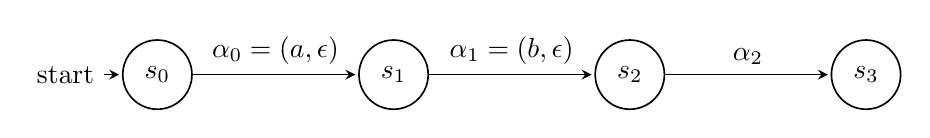
\begin{tikzpicture}[->,shorten >=1pt,node distance=3cm,on
      grid,auto,scale=.5,semithick,>=stealth]
			\node[state,initial] (s0) {$s_0$};
      \node[state] (s1) [right of=s0] {$s_1$};
      \node[state] (s2) [right of=s1] {$s_2$};
      \node[state] (s3) [right of=s2] {$s_3$};
			\path
				(s0) edge node {$\alpha_0 = (a, \epsilon)$} (s1)
				(s1) edge node {$\alpha_1 = (b, \epsilon)$} (s2)
				(s2) edge node {$\alpha_2$} (s3);
		\end{tikzpicture}
    \subcaption{The system model $M$ consisting of two function calls, to $a$
    and $b$, and an unspecified event $\alpha_2$.}
	\end{minipage}

  \bigskip

	\begin{minipage}{0.90\textwidth}
		\centering
		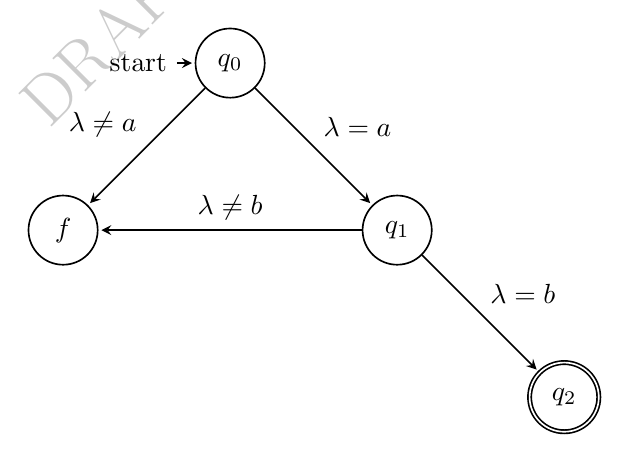
\begin{tikzpicture}[->,shorten >=1pt,node distance=3cm,on
      grid,auto,scale=.5,semithick,>=stealth]
			\node[state,initial] (q0) {$q_0$};
      \node[state] (q1) [below right of=q0] {$q_1$};
      \node[state] (f) [below left of=q0] {$f$};
      \node[state,accepting] (q2) [below right of=q1] {$q_2$};
			\path
        (q0) edge node {$\lambda = a$} (q1)
        (q0) edge node [above left] {$\lambda \neq a$} (f)
        (q1) edge node {$\lambda = b$} (q2)
        (q1) edge node [above] {$\lambda \neq b$} (f);
		\end{tikzpicture}
    \subcaption{The specification automata $C$. This automata is designed to
      accept system models that consists of one call to $a$ followed by a call to
      $b$. After that, verification is complete and any events are accepted.
      $f$ is a fail state and $q_2$ is a success state.}
	\end{minipage}

  \bigskip

	\begin{minipage}{0.90\textwidth}
		\centering
		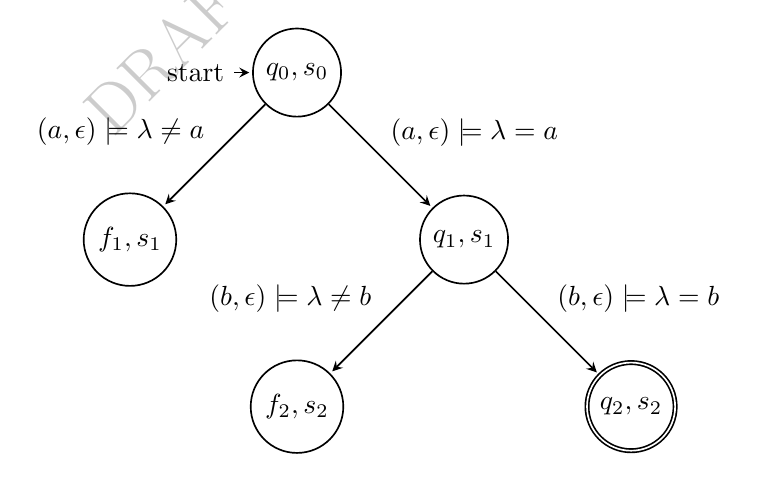
\begin{tikzpicture}[->,shorten >=1pt,node distance=3cm,on
      grid,auto,scale=.5,semithick,>=stealth]
			\node[state,initial] (q0) {$q_0,s_0$};
      \node[state] (q1) [below right of=q0] {$q_1,s_1$};
      \node[state] (f1) [below left of=q0] {$f_1,s_1$};
      \node[state,accepting] (q2) [below right of=q1] {$q_2,s_2$};
      \node[state] (f2) [below left of=q1] {$f_2,s_2$};
			\path
        (q0) edge node {$(a, \epsilon) \models \lambda = a$} (q1)
        (q0) edge node [above left] {$(a, \epsilon) \models \lambda \neq a$} (f1)
        (q1) edge node {$(b, \epsilon) \models \lambda = b$} (q2)
        (q1) edge node [above left] {$(b, \epsilon) \models \lambda \neq b$} (f2);
		\end{tikzpicture}
    \subcaption{The product of the model and the specification, $M \times C$.
    $(f_1,s_1)$ and $(f_2,s_2)$ are fail states; $(q_2,s_2)$ is a success state.}
	\end{minipage}

  \caption{Deduction example.}
	\label{figure-deduction-example}
\end{figure}
%%%%%%%%%%%%%%%%%%%%%%%%
%%%%%%%%%%%%%%%%%%%%%%%%
%%%%%%%%%%%%%%%%%%%%%%%%


\subsubsection{Evaluating specification-model product label expressions}

The transition labels for the product of a specification automata and a system
model is of the form (the second line is a expanded form of the first):

\medskip
\[
  \begin{array}{rcl}
    \alpha & \models & \text{expression $E$ over $\alpha$} \\
    (\lambda, \delta) & \models & \text{expression $E$ over $\lambda$ and $\delta$}
  \end{array}
\]
\medskip

The expression $E$ is translated directly from Python expressions in the
specification function. An incomplete sketch of the translation procedure,
shown in Figure~\ref{figure-semantics-translation}, is just syntax replacement.
The resulting specification expression has the same semantics as the Python
expression. In the same way that the Python specification operates on an event,
a specification expression is evaluated to true ($\top$) or false ($\bot$)
using the values of an event $\alpha$.

\begin{figure}[h!]
	\begin{minipage}{0.9\textwidth}
		\centering
    \begin{tabular}{r c l}
      $PE(\texttt{True)})$ & = & $\top$ \\
      $PE(\texttt{False)})$ & = & $\bot$ \\
      $PE(\texttt{event.fn.x.called})$ & = & $\lambda = x$ \\
      $PE(\texttt{event.called\_function == x})$ & = & $\lambda = x$ \\
      $PE(\texttt{event.fn.x.property})$ & = & $\delta(x.\texttt{property})$ \\
      $PE(\texttt{not a)})$ & = & $\neg PE(\texttt{a})$ \\
      $PE(\texttt{a == b)})$ & = & $PE(\texttt{a}) = PE(\texttt{b})$ \\
      $PE(\texttt{a != b)})$ & = & $PE(\texttt{a}) \neq PE(\texttt{b})$ \\
      $PE(\texttt{a and b)})$ & = & $PE(\texttt{a}) \wedge PE(\texttt{b})$ \\
      $PE(\texttt{a or b)})$ & = & $PE(\texttt{a}) \vee PE(\texttt{b})$ \\
      $PE(\textit{A Python function or property})$ & = & \textit{The return value} \\
    \end{tabular}
  \end{minipage}
  \caption{A sketch of the translation procedure of Python expressions to
    specification expressions. $PE$ is the mapping function, replacing the
    Python syntax with mathematics syntax.}
  \label{figure-semantics-translation}
\end{figure}


\subsubsection{Verification}

A product $Z$ of a system model and a specification can be used to determine
whether that specification would accept or reject the system model --- or not
know to do either or, yet.

\begin{enumerate}
  \item Compute the product $Z$ of the specification $C$ and the system model
    $M$, as described above.

  \item Traverse $Z$, starting at the root node, following all transitions
    which labels evaluate to true.

    \begin{enumerate}
      \item If a fail state is reached, the system models violates the
        specification.
      \item If only success states are reached, the system model satisfies the
        specification.
      \item If some traversal ends in a state that is neither a fail or a
        success state, the system model could, if it were extended, either
        satisfy or violate the specification.
    \end{enumerate}
\end{enumerate}

Formal \textit{pythonrv} specifications are verified using this procedure,
although in an incremental manner. The verification is done online, so as soon
as a new event is added to the system model, it is combined with the
specification automata.

We now go on to describe the actual syntax for these formal specification
functions.


\subsection{Python Subset for Formal Specification Functions}
\label{section-approach-python-subset}
\lstset{language=Python,numbers=left}

The subset of Python that can be used in formal \textit{pythonrv} specification
functions consists of three composable specification functions:
\textit{assert}, \textit{next} and \textit{if}; See
Figure~\ref{figure-basic-formal-specification-functions}. A complete and
verifiable formal specification function also needs some boilerplate, shown in
Figure~\ref{figure-formal-boilerplate}.

\begin{figure}[h!]
	\begin{center}
	\begin{minipage}{0.7\textwidth}
	\begin{lstlisting}
def spec():
  a = make_assert(E)
  tail = # optional composition point 'tail'
  return a + tail

def next():
  x = # required composition point 'next'
  n = make_next(x)
  tail = # optional composition point 'tail'
  return n + tail

def if():
  then = # required composition point 'then'
  els = # optional composition point 'else'
  i = make_if(E, then, else)
  tail # optional composition point 'tail'
  return i + tail
	\end{lstlisting}
	\end{minipage}
	\end{center}

	\caption{The three basic formal specification functions.}
	\label{figure-basic-formal-specification-functions}
\end{figure}

\begin{figure}[h!]
	\begin{center}
	\begin{minipage}{0.7\textwidth}
	\begin{lstlisting}
from pythonrv import rv
from pythonrv.formalrv import (formal_spec,
  make_assert, make_next, make_if)

monitorees = # list of monitorees
@rv.monitor(monitorees)
@formal_spec
def spec():
  # spec is a formal specification function
  # - assert, next or if
	\end{lstlisting}
	\end{minipage}
	\end{center}

  \caption{The boilerplate code for formal \textit{pythonrv} specification
  functions that allow verification and instrumentation to take place.}
	\label{figure-formal-boilerplate}
\end{figure}

The label \textit{E} used in the assertion and if statement (lines 2 and 11)
denotes any idempotent, immutable, valid Python boolean expression. A technical
detail is that if the expression needs to access any properties of the
\texttt{event} argument, they need to be of the form \texttt{lambda event: E}.
The previous section described how these expressions are used in formal
verification.

The three basic formal specification functions correspond to simple,
nondeterministic, finite automata, which are depicted in
Figure~\ref{figure-basic-formal-specification-automata}. The basic formal
specifications can be combined by composition into larger, more complex
specifications. Details on the basic formal specification functions and their
composition is described in the next section. Note that the \textit{assert}
formal specification function, and all complete compositions of the three basic
formal specification functions, are valid \textit{pythonrv} specification
functions.

%%%%%%%%%%%%%%%%%%%%%%%%
%% Automata for the basic formal specification functions
%%%%%%%%%%%%%%%%%%%%%%%%
\begin{figure}[h!]
	\begin{minipage}{0.45\textwidth}
		\centering
		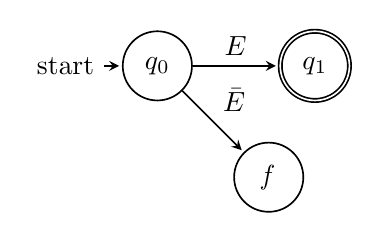
\begin{tikzpicture}[->,shorten >=1pt,node distance=2cm,on
      grid,auto,scale=.5,semithick,>=stealth]
			\node[state,initial] (q0) {$q_0$};
			\node[state,accepting] (q1) [right of=q0] {$q_1$};
      \node[state] (f) [below right of=q0] {\textit{f}};
			\path
				(q0) edge node {$E$} (q1)
        (q0) edge node {$\bar{E}$} (f);
		\end{tikzpicture}
    \subcaption{A generalized \textit{assert} specification, asserting the
      expression $E$. $q_1$ is a success state; \textit{f} is a fail state.}
	\end{minipage}
  ~
	\begin{minipage}{0.45\textwidth}
		\centering
		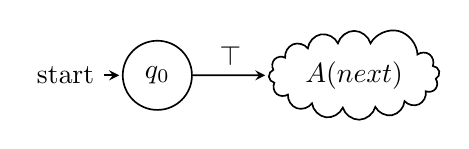
\begin{tikzpicture}[->,shorten >=1pt,node distance=2.5cm,on
      grid,auto,scale=.5,semithick,>=stealth]
			\node[state,initial] (q0)	{$q_0$};
			\node[cloud, cloud puffs=15.7, cloud ignores aspect, align=center, draw] (cloud) [right of=q0] {$A(next)$};
			\path
				(q0) edge node {$\top$} (cloud);
		\end{tikzpicture}
    \subcaption{A template for a \textit{next} specification.}
	\end{minipage}

  \bigskip

	\begin{minipage}{0.90\textwidth}
		\centering
		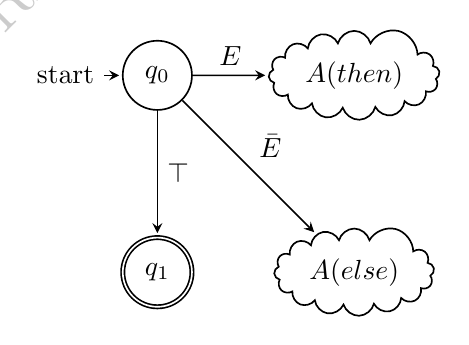
\begin{tikzpicture}[->,shorten >=1pt,node distance=2.5cm,on
      grid,auto,scale=.5,semithick,>=stealth]
			\node[state,initial] (q0)	{$q_0$};
			\node[cloud, cloud puffs=15.7, cloud ignores aspect, align=center, draw] (then) [right of=q0] {$A(then)$};
			\node[cloud, cloud puffs=15.7, cloud ignores aspect, align=center, draw] (else) [below of=then] {$A(else)$};
			\node[state,accepting] (q1) [below of=q0]	{$q_1$};
			\path
				(q0) edge node {$E$} (then)
        (q0) edge node {$\bar{E}$} (else)
        (q0) edge node {$\top$} (q1);
		\end{tikzpicture}
    \subcaption{A template for an \textit{if} specification.}
	\end{minipage}

  \caption{Sketches of automata for the three basic formal specification
    functions. The squiggles around $A(next)$, $A(then)$ and $A(else)$ denote
    that some composition is required there.}
	\label{figure-basic-formal-specification-automata}
\end{figure}
%%%%%%%%%%%%%%%%%%%%%%%%
%%%%%%%%%%%%%%%%%%%%%%%%
%%%%%%%%%%%%%%%%%%%%%%%%


\subsection{Transformation to Automata and Rules for Composition}
\label{section-approach-composition}
\lstset{language=Python,numbers=none}

The idea is to use composition to build more complex and interesting
specifications from the three basic formal specification functions. Composition
is defined inductively, preserving the semantics from
Section~\ref{section-approach-semantics}.

There are no implicit precedence rules for the $\circ$ composition operator;
parentheses are required.


\subsubsection{Composition of the \textit{assert} specification, and
composition with the \textit{tail} composition point}

The \textit{assert} specifications are the only basic formal specification
functions that are complete, without the need to compose them with other
specifications. The automata $A(a_E)$ for a standalone \textit{assert}
specification $a_E$, depicted in
Figure~\ref{figure-basic-formal-specification-automata}~(a), is defined as:

\medskip
\[
  \begin{array}{rcl}
    A(a_E) & = & (\{q_0, q_1, f\}, \{(q_0, q_1, E), (q_0, f, \bar{E})\}, q_0, \{q_1\}, \{f\})
  \end{array}
\]
\medskip

If $\bar{E}$ is true, the fail state $f$ will be reached, and the specification
has been violated.

\textit{assert} specifications also have, together with all basic formal
specification functions and compositions thereof, at least one open composition
point, the \textit{tail} composition point. Compositions using the
\textit{tail} composition point are commutative: $s \, \circ_{tail} \, s' = s'
\, \circ_{tail} \, s$. Composition using the \textit{tail} composition point is
essentially just a merge of the initial states of the two specifications,
making the initial transitions of both specifications go out from the same
state $q_0$, and merging the success states and fail states of the automata. Given two
specifications $s$ and $s'$, where:

\medskip
\[
  \begin{array}{rcl}
    A(s) & = & (Q_s, T_s \cup R_s, q_{0s}, S_s, F_s) \\
   A(s') & = & (Q_{s'}, T_{s'} \cup R_{s'}, q_{0s'}, S_{s'}, F_{s'})
  \end{array}
\]
\medskip

Then:

\medskip
\[
  \begin{array}{rcl}
    A(s \circ_{tail} s') & = & (Q, P, q_0, S_s \cup S_{s'}, F_s \cup F_{s'}) \\
                       Q & = & \{q_0\} \cup Q_s \cup Q_{s'} - \{q_{0s}, q_{0s'}\} \\
                       P & = & T \cup R_s \cup R_{s'} \\
                       T & = & \{(q_0, q', E) \, | \, (q, q', E) \in (T_s \cup T_{s'})\} \\
  \end{array}
\]
\medskip

An example for composing two \textit{assert} specifications is shown in
Figure~\ref{figure-assert-composition-example}. The resulting automata is
unnecessarily complex, and can be simplified to a smaller automata with the
same semantics, as seen in Figure~\ref{figure-assert-composition-simplified}.


%%%%%%%%%%%%%%%%%%%%%%%%
%% Composition, assert o s, symbol-python-automata
%%%%%%%%%%%%%%%%%%%%%%%%
\begin{figure}[h!]
	\begin{minipage}{0.90\textwidth}
		\centering
    \[
      \begin{array}{rcl}
        A(a_E) & = & (\{q_x, q_y, f\}, \{(q_x, q_y, E), (q_x, f, \bar{E})\}, q_x, \{q_y\}, \{f\}) \\
    A(a'_{E'}) & = & (\{q_z, q_w, f'\}, \{(q_z, q_w, E') ,(q_z, f', \bar{E'})\}, q_z, \{q_w\}, \{f'\})
      \end{array}
    \]
		\centering
    \[
      \begin{array}{rcl}
        A(a_E \circ_{tail} a'_{E'}) & = & (Q, P, q_0, S, F) \\
                                 Q & = & \{q_0, q_y, f, q_w, f'\} \\
                                 P & = & \{(q_0, q_y, E), (q_0, f, \bar{E}), (q_0, q_w, E'), (q_0, f', \bar{E'})\} \\
                                 S & = & \{q_y, q_w\} \\
                                 F & = & \{f, f'\}
      \end{array}
    \]
	\end{minipage}

  \bigskip

	\begin{minipage}{0.45\textwidth}
		\centering
    \begin{lstlisting}
def s():
  return make_assert(E) +
         make_assert(E')
    \end{lstlisting}
	\end{minipage}
  ~
	\begin{minipage}{0.45\textwidth}
		\centering
		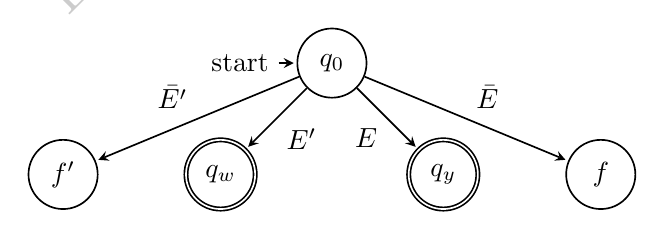
\begin{tikzpicture}[->,shorten >=1pt,node distance=2cm,on
      grid,auto,scale=.5,semithick,>=stealth]
			\node[state,initial] (q0) {$q_0$};
			\node[state,accepting] (qy) [below right of=q0] {$q_y$};
			\node[state] (f) [right of=qy] {$f$};
			\node[state,accepting] (qw) [below left of=q0] {$q_w$};
			\node[state] (f') [left of=qw] {$f'$};
			\path
        (q0) edge node [below left] {$E$} (qy)
        (q0) edge node [below right] {$E'$} (qw)
        (q0) edge node [above right] {$\bar{E}$} (f)
        (q0) edge node [above left] {$\bar{E'}$} (f');
		\end{tikzpicture}
	\end{minipage}
  \caption{An example showing a composition of an \textit{assert} specification
    $a_E$ with another \textit{assert} specification $a'_{E'}$. Only the
    resulting $A(a_E \, \circ_{tail} \, a'_{E'})$ automata is shown. $q_y$ and
    $q_w$ are success states; $f$ and $f'$ are fail states.}
	\label{figure-assert-composition-example}
\end{figure}

\begin{figure}[h!]
	\begin{minipage}{0.45\textwidth}
		\centering
    \[
      (\{q_0, q_1, f\}, \{(q_0, q_1, E \wedge E'), (q_0, f, \bar{E} \vee \bar{E'})\}, q_0, \{q_1\}, \{f\})
    \]
	\end{minipage}
	\begin{minipage}{0.45\textwidth}
		\centering
		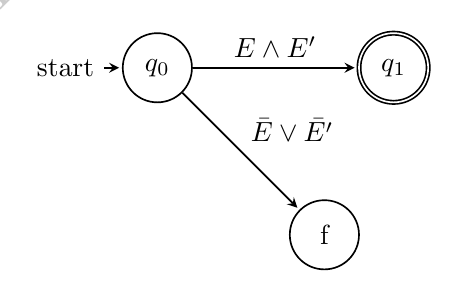
\begin{tikzpicture}[->,shorten >=1pt,node distance=3cm,on
      grid,auto,scale=.5,semithick,>=stealth]
			\node[state,initial] (q0) {$q_0$};
			\node[state,accepting] (q1) [right of=q0] {$q_1$};
			\node[state] (f) [below right of=q0] {f};
			\path
				(q0) edge node {$E \wedge E'$} (q1)
        (q0) edge node {$\bar{E} \vee \bar{E'}$} (f);
		\end{tikzpicture}
	\end{minipage}
  \caption{A simplified version of the automata from
    Figure~\ref{figure-assert-composition-example}, semantically identical. The
  success states have been merged into $q_1$, and the fail states into $f$.}
	\label{figure-assert-composition-simplified}
\end{figure}

%%%%%%%%%%%%%%%%%%%%%%%%
%%%%%%%%%%%%%%%%%%%%%%%%
%%%%%%%%%%%%%%%%%%%%%%%%


\subsubsection{Composition of the \textit{next} specification}

The \textit{next} specification functions are the specifications that deal with
time.  \textit{next} specifications have two composition points: one
appropriately called \textit{next}, which is required, and one called
\textit{tail}, which is optional. Composition using the \textit{tail}
composition point was described above.

Composition with the \textit{next} composition point, $n \, \circ_{next} \, s$
with $A(s) = (Q, P, q_0, S, F)$ is as follows:

\medskip
\[
  \begin{array}{rcl}
    A(n \circ_{next} s) & = & (\{q_0'\} \cup Q, T \cup P, q_0', S, F) \\
               T  & = & \{(q_0', q_0, \top)\}
  \end{array}
\]
\medskip

This is illustrated in Figure~\ref{figure-next-composition-s}.

Also note that composition using the \textit{next} composition point is
associative, as shown in Figure~\ref{figure-next-associative}.



%%%%%%%%%%%%%%%%%%%%%%%%
%% Composition, next o s, symbol-python-automata
%% Associativity of the next composition point
%%%%%%%%%%%%%%%%%%%%%%%%
\begin{figure}[h!]
	\begin{minipage}{0.20\textwidth}
		\centering
    \[
      s' = n \, \circ_{next} \, s
    \]
	\end{minipage}
  ~
	\begin{minipage}{0.35\textwidth}
		\centering
    \begin{lstlisting}
def s'():
  return make_next(s)
    \end{lstlisting}
	\end{minipage}
  ~
	\begin{minipage}{0.4\textwidth}
		\centering
		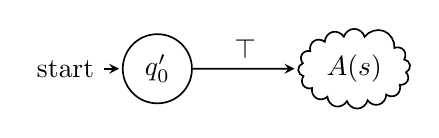
\begin{tikzpicture}[->,shorten >=1pt,node distance=2.5cm,on
      grid,auto,scale=.5,semithick,>=stealth]
			\node[state,initial] (q0')	{$q_0'$};
			\node[cloud, cloud puffs=15.7, cloud ignores aspect, align=center, draw] (cloud) [right of=q0'] {$A(s)$};
			\path
				(q0') edge node {$\top$} (cloud);
		\end{tikzpicture}
	\end{minipage}
  \caption{The composition of a \textit{next} specification with any
    specification $s$, using the \textit{next} composition point.}
	\label{figure-next-composition-s}
\end{figure}

\begin{figure}[h!]
	\begin{minipage}{0.9\textwidth}
		\centering
    \[
      \begin{array}{rcl}
        (n \, \circ_{next} \, s_1) \, \circ_{tail} \, (n' \, \circ_{next} \, s_2)
        & = & n \, \circ_{next} \, t \\
        t & = & s_1 \, \circ_{tail} \, s_2
      \end{array}
    \]
	\end{minipage}

  \bigskip

	\begin{minipage}{0.45\textwidth}
		\centering
    \begin{lstlisting}
def s():
  return make_next(s1) +
    make_next(s2)

# equivalent to
def s():
  return make_next(t)

def t(event):
  return s1() + s2()
    \end{lstlisting}
	\end{minipage}
  ~
	\begin{minipage}{0.45\textwidth}
		\centering
		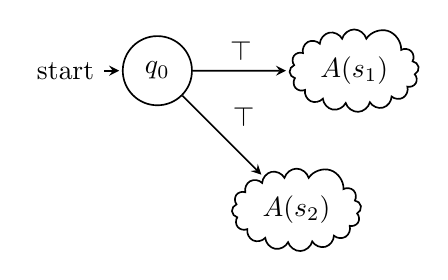
\begin{tikzpicture}[->,shorten >=1pt,node distance=2.5cm,on
      grid,auto,scale=.5,semithick,>=stealth]
			\node[state,initial] (q0)	{$q_0$};
			\node[cloud, cloud puffs=15.7, cloud ignores aspect, align=center, draw] (s1) [right of=q0] {$A(s_1)$};
			\node[cloud, cloud puffs=15.7, cloud ignores aspect, align=center, draw] (s2) [below right of=q0] {$A(s_2)$};
			\path
				(q0) edge node {$\top$} (s1)
				(q0) edge node {$\top$} (s2);
		\end{tikzpicture}

    \bigskip

		\centering
		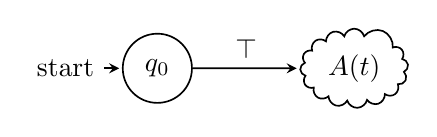
\begin{tikzpicture}[->,shorten >=1pt,node distance=2.5cm,on
      grid,auto,scale=.5,semithick,>=stealth]
			\node[state,initial] (q0) {$q_0$};
			\node[cloud, cloud puffs=15.7, cloud ignores aspect, align=center, draw] (t) [right of=q0] {$A(t)$};
			\path
				(q0) edge node {$\top$} (t);
		\end{tikzpicture}
	\end{minipage}
  \caption{The associativity of the \textit{next} composition point in a
  \textit{next} formal specification function.}
	\label{figure-next-associative}
\end{figure}
%%%%%%%%%%%%%%%%%%%%%%%%
%%%%%%%%%%%%%%%%%%%%%%%%
%%%%%%%%%%%%%%%%%%%%%%%%


\subsubsection{Composition of the \textit{if} specification}

\textit{if} specifications have three composition points: one required,
\textit{then}, and two optional, \textit{else} and \textit{tail}. Composition
using the \textit{tail} composition point was described above.

In an \textit{if} specification $i_E$ we consider the expression $E$ as a guard
for the \textit{then} composition point, and $\bar{E}$ as a guard for the
\textit{else} composition point.

The composition essentially becomes to add the guard $E$ to the labels of all
initial transitions for the automata at the \textit{then} composition point,
and $\bar{E}$ to the labels of all initial transitions for the automata at the
\textit{else} composition point. The guards, $E$ and $\bar{E}$ are added as
parts of a conjunctive.

Let $s_1$ be the specification attached to the \textit{then} composition point
and an optional $s_2$ attached to the \textit{else} composition point, and
$A(s_1) = (Q_1, T_1 \cup R_1, q_{10}, S_1, F_1)$, $A(s_2) = (Q_2, T_2 \cup R_2,
q_{20}, S_2, F_2)$. Then:

\medskip
\[
  \begin{array}{rcl}
  A((i_E \circ_{then} s_1) \circ_{else} s_2) & = & (Q, P, q_0, S, F) \\
                                           Q & = & Q_1 \cup Q_2 \cup \{q_0, q_1\} - \{q_{10}, q_{20}\} \\
                                           P & = & T'_1 \cup T'_2 \cup R_1 \cup R_2 \cup X \\
                                        T'_1 & = & \{(q_0, q, E       \wedge E') \, | \, (q_{10}, q, E') \in T_1\} \\
                                        T'_2 & = & \{(q_0, q, \bar{E} \wedge E') \, | \, (q_{20}, q, E') \in T_2\} \\
                                           X & = & \{(q_0, q_1, \top)\} \\
                                           S & = & S_1 \cup S_2 \cup \{q_1\} \\
                                           F & = & F_1 \cup F_2
  \end{array}
\]
\medskip

If the \textit{else} composition point is left out, then $Q_2 = T_2 = R_2 = S_2
= F_2 = \emptyset$. $X$ is the fall-through transition to the success state
$q_1$, which can always be reached. This will allow for successful verification
when $E$ is false and there is no else clause.

With these constructions in mind, the next section shows a few functioning
examples.


\subsection{Examples of Formal Specifications}
\label{section-approach-examples-of-formal-specifications}
\lstset{language=Python,numbers=none}

Here follows two examples of formal \textit{pythonrv} specifications, both in
their specification function form, written in Python and shown in
Figure~\ref{figure-formal-syntax-example-1} and
Figure~\ref{figure-formal-syntax-example-2}, and as automata, shown in
Figure~\ref{figure-formal-syntax-example-1-automata} and
Figure~\ref{figure-formal-syntax-example-2-automata}.

The first example, Figure~\ref{figure-formal-syntax-example-1}
and~\ref{figure-formal-syntax-example-1-automata}, shows a simple specification
that makes sure that the first argument to the function \texttt{fib} in the
module \texttt{fibmodule} is always positive. The main difference with the
similar informal specification in Figure~\ref{figure-syntax-example-1} is that
here we have to explicitly create a loop by composing with a \textit{next}
specification, pointing back to \texttt{spec}. This is required so that not
only the first event is verified.

The example in Figure~\ref{figure-formal-syntax-example-2} is more complex, as
can be seen by the sprawling automata in
Figure~\ref{figure-formal-syntax-example-2-automata}. The specification
verifies accepts only interleaving calls to two functions, starting with
\texttt{mymodule.foo}, then to \texttt{mymodule.bar}. This is represented by
the loop between the $q_0$ and $r_0$ states in the automata. Because the labels
for the transitions between them are $\top$, i.e.\ always true, we are
guaranteed that on every event we either transition into state $q_0$ or $q_1$,
and verification will never be finished. The specification also asserts that if
\texttt{foo} is called with $0$ as the first argument, the second argument must
also be $0$. This is just to demonstrate how the \textit{if} construct works.


%%%%%%%%%%%%%%%%%%%%%%%%
%% formal syntax examples
%%%%%%%%%%%%%%%%%%%%%%%%
\begin{figure}[h!]
	\begin{center}
	\begin{minipage}{0.9\textwidth}
	\lstinputlisting{figures/formal_syntax_example_1.py}
	\end{minipage}
	\end{center}

  \caption{A formal \textit{pythonrv} specification function, similar to the
    informal specification function shown in
    Figure~\ref{figure-syntax-example-1}. The automata for this specification
    function is shown in Figure~\ref{figure-formal-syntax-example-1-automata}.}
	\label{figure-formal-syntax-example-1}
\end{figure}

\begin{figure}[h!]
	\begin{minipage}{0.9\textwidth}
		\centering
    \[
      \begin{array}{rcl}
        A(\text{spec}) & = & (Q, P, q_0, S, F) \\
                     Q & = & \{q_0, q_1, f\} \\
                     P & = & \{(q_0, q_1, \delta(\texttt{func.inputs$[0]$}) > 0),
      (q_0, f, \neg(\delta(\texttt{func.inputs$[0]$}) > 0)), \\
                       &   & \; (q_0, q_0, \top)\} \\
                     S & = & \{q_1\} \\
                     F & = & \{f\}
      \end{array}
    \]
	\end{minipage}

  \bigskip

	\begin{minipage}{0.9\textwidth}
		\centering
		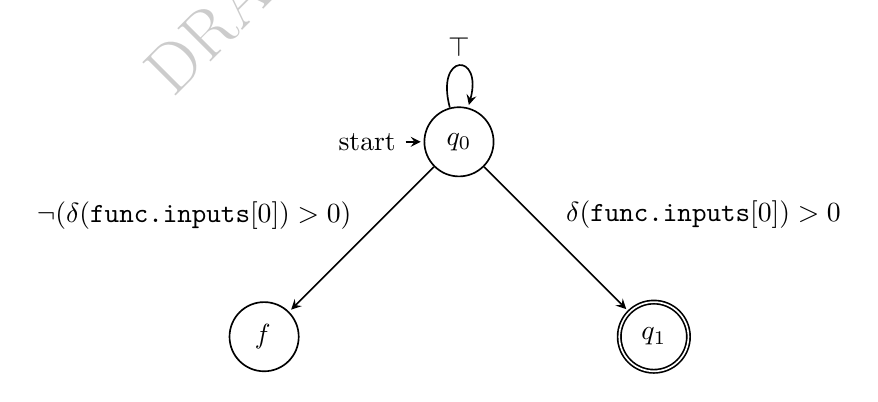
\begin{tikzpicture}[->,shorten >=1pt,node distance=3.5cm,on
      grid,auto,scale=.5,semithick,>=stealth]
			\node[state,initial] (q0) {$q_0$};
			\node[state,accepting] (q1) [below right of=q0] {$q_1$};
      \node[state] (f) [below left of=q0] {\textit{f}};
			\path
        (q0) edge [loop above] node {$\top$} (q0)
        (q0) edge node {$\delta(\texttt{func.inputs$[0]$}) > 0$} (q1)
        (q0) edge node [above left] {$\neg(\delta(\texttt{func.inputs$[0]$}) > 0)$} (f);
		\end{tikzpicture}
	\end{minipage}
  \caption{The automata for the formal \textit{pythonrv} specification function
    in Figure~\ref{figure-formal-syntax-example-1}.}
	\label{figure-formal-syntax-example-1-automata}
\end{figure}

\begin{figure}[h!]
	\begin{center}
	\begin{minipage}{0.9\textwidth}
	\lstinputlisting{figures/formal_syntax_example_2.py}
	\end{minipage}
	\end{center}

  \caption{A more complex formal \textit{pythonrv} specification function. The automata for
    this specification function is shown in
    Figure~\ref{figure-formal-syntax-example-2-automata}.}
	\label{figure-formal-syntax-example-2}
\end{figure}

\begin{figure}[h!]
	\begin{minipage}{0.9\textwidth}
		\centering
    \[
      \begin{array}{rcl}
        A(\text{spec}) & = & (Q, P_1 \cup P_2 \cup P_3 \cup P_4, q_0, S, F) \\
                     Q & = & \{q_0, q_1, f_1, q_2, q_3, f_2, r_0, r_1, f_r\} \\
                   P_1 & = & \{(q_0, q_1, \lambda = \texttt{foo}), (q_0, f_1, \neg(\lambda = \texttt{foo}))\} \\
                   P_2 & = & \{(q_0, q_2, G \wedge X), (q_0, f_2, G \wedge \neg X), (q_0, q_3, \top)\} \\
                   P_3 & = & \{(q_0, r_0, \top), (r_0, q_0, \top)\} \\
                   P_4 & = & \{(r_0, r_1, \lambda = \texttt{bar}), (r_0, f_r, \neg(\lambda = \texttt{bar}))\} \\
                     S & = & \{q_1, q_2, q_3, r_1\} \\
                     F & = & \{f_1, f_2, f_r\} \\
                     G & = & \delta(\texttt{foo.inputs$[0]$}) = 0 \\
                     X & = & \delta(\texttt{foo.inputs$[1]$}) = 0
      \end{array}
    \]
	\end{minipage}

  \bigskip

	\begin{minipage}{0.9\textwidth}
		\centering
		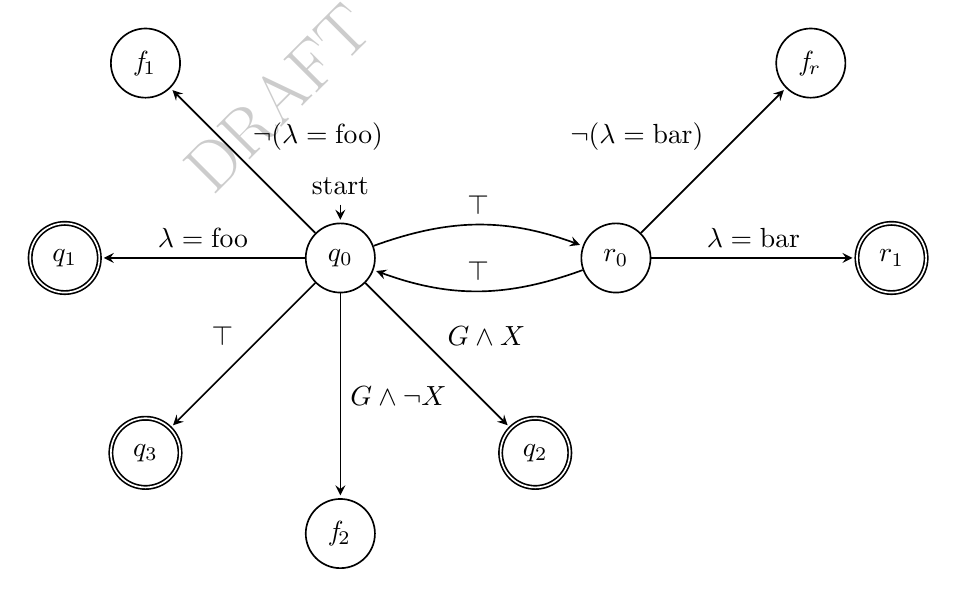
\begin{tikzpicture}[->,shorten >=1pt,node distance=3.5cm,on
      grid,auto,scale=.5,semithick,>=stealth]

      % first spec
			\node[state,initial above] (q0) {$q_0$};
			\node[state,accepting] (q1) [left of=q0] {$q_1$};
      \node[state] (f1) [above left of=q0] {\textit{f$_1$}};
      % if
			\node[state,accepting] (q2) [below right of=q0] {$q_2$};
      \node[state] (f2) [below of=q0] {\textit{f$_2$}};
			\node[state,accepting] (q3) [below left of=q0] {$q_3$};

      % second spec
      \node[state] (r0) [right of=q0] {$r_0$};
			\node[state,accepting] (r1) [right of=r0] {$r_1$};
      \node[state] (fr) [above right of=r0] {\textit{f$_r$}};
			\path
        % first spec
        % assert
        (q0) edge node [above] {$\lambda = \text{foo}$} (q1)
        (q0) edge node [above right] {$\neg(\lambda = \text{foo})$} (f1)
        % if
        (q0) edge node [above right] {$G \wedge X$} (q2)
        (q0) edge node [right] {$G \wedge \neg X$} (f2)
        (q0) edge node [above left] {$\top$} (q3)
        % next
        (q0) edge [bend left=20] node [above] {$\top$} (r0)

        % second spec
        % assert
        (r0) edge node {$\lambda = \text{bar}$} (r1)
        (r0) edge node [above left] {$\neg(\lambda = \text{bar})$} (fr)
        % next
        (r0) edge [bend left=20] node [above] {$\top$} (q0);
		\end{tikzpicture}
	\end{minipage}
  \caption{A direct translation of the formal \textit{pythonrv} specification
    function in Figure~\ref{figure-formal-syntax-example-2} to an automata.
    $q_0$ is the root for the \texttt{spec} specification, and $r_0$ is the
    root of the \texttt{spec\_bar\_called} specification. $q_1$ and $f_1$
    relates to the assertion in \texttt{spec}, and $q_2$, $q_3$ and $f_2$ to
    the if statement. $r_1$ and $f_r$ relates to the assertion in
    \texttt{spec\_bar\_called}.}
	\label{figure-formal-syntax-example-2-automata}
\end{figure}
%%%%%%%%%%%%%%%%%%%%%%%%
%%%%%%%%%%%%%%%%%%%%%%%%
%%%%%%%%%%%%%%%%%%%%%%%%


%================================================
%====== Chapter 6, Evaluation
%================================================

\pagestyle{newchap}
\chapter{Evaluation} \label{chapter-evaluation}

To see how \textit{pythonrv} would work in a real-world setting it was
incorporated into a real-time web application for Valtech Sweden, a
medium-sized Swedish company.

The web application is written in Python 2.7 using the
Django\footnote{\texttt{https://www.djangoproject.com/}} web framework. It has
approximately 10000 lines of code.

There are two questions we need to answer when writing specifications for a
program. First, when, in the life-cycle of the program, should we attach the
specifications? In other words, when should the code instrumentation be done?
And second, and most important: what specifications should be written, and for
which functions?

We can answer the first question first. It requires a bit of knowledge on the
start up sequence for, and structure of, Django applications.


\section{Technical Perspective}


\subsection{Anatomy of a Django Application}

A Django application follows the Model-View-Controller pattern, or as they call
it, the Model-Template-View pattern. The model is a representation of the data
used by the program, and the templates are the layer that constructs the
display for the user. The view links the two together, fetching the correct
models for specific requests, and then delegating to the appropriate templates.

Application-specific configuration for Django programs are stored in settings
modules, which are ordinary Python files. These contain settings for database
connections, authentication, etc. During startup, Django reads the settings
files, starts up its internal machinery, and waits for the first request.


\subsection{When to Attach}

At first glance it might seem desirable to attach the specifications before
even starting the Django framework. That way we could monitor the startup
process, and all of the functionality of Django.

A problem with this, that is due to how Python works, and how \textit{pythonrv}
does code instrumentation, is that \textit{pythonrv} needs to load the modules
(files) for each function to be monitored. These modules are often heavily
dependent on Django, and that it has been started correctly, with all settings
loaded.

A suitable time to instrument the program --- to enable the specifications ---
is during startup, after the settings have been loaded. Some specifications,
which do not monitor code dependent on the settings, could be loaded before
that.


\subsection{Technical Issues}

Early in the process of using \textit{pythonrv} in the web application it was
discovered that the copying of data, such as function arguments, that
\textit{pythonrv} does would not work with Django. The latest version of
Django, v1.4.1, uses a module called \texttt{cStringIO}, which produces objects
that cannot be copied. All functions dealing with web requests are affected by
this. This has been fixed in the development branch of Django, but in the
meantime, \textit{pythonrv} has an option to disable argument copying, either
for all specifications or for a subset of them, to work around this issue.


\section{Potential Value}

Now to the most important question: what specifications could, and should, be
written? What value do they provide?

The web application is only intended for internal use, for employees.
Authentication of employees and authorization of their access rights are very
important. Specifications can be written to make sure all views or requests are
made by an authenticated user (except for the login screen), and that they are
allowed to perform the requested action. A specification showing a
specification verifying that proper authentication has been done is shown in
Figure~\ref{figure-app-authentication-informal}. This is just one way of
writing a specification function for this requirement. There are several other
options, such as utilizing the temporal capabilities of runtime verification
with the \texttt{event.next} function. E.g., if a request asks for a resource
requiring authentication, we could specify that before the response is sent,
authentication must have been done.

\begin{figure}[h!]
	\begin{center}
	\begin{minipage}{0.9\textwidth}
	\lstinputlisting{figures/app_authentication_informal.py}
	\end{minipage}
	\end{center}

  \caption{An informal \textit{pythonrv} specification verifying that views are
    only accessible with proper authentication. Note how the use of Python in
    the specification function allows us to refactor away the condition that
    determines whether authentication should be required, leaving the
    specification much simpler and cleaner.}
	\label{figure-app-authentication-informal}
\end{figure}

\todo{more examples}
Talk about where specifications would be suitable, and for what.





%================================================
%====== Chapter 7, Conclusions
%================================================

\pagestyle{newchap}
\chapter{Conclusions} \label{chapter-conclusions}

This report, and the proof-of-concept implementation \textit{pythonrv}, has
shown that it is possible to write specifications in the target programs
programming language (Python) and in a manner more similar to unit testing.

\todo{excitement! and better structure}

However, a few reservations should be mentioned.

The specification functions' explicit dealing with time and the actual
execution flow leads to some inherent divergences from ordinary unit testing
styles. This is best exemplified by the \texttt{event.next} method described in
Chapter~\ref{chapter-approach}. Expectations could perhaps help here, see the
next section.

Also, giving the specifications a formal foundation, and doing formal
verification with them, is different and difficult, than with specifications
already written in formal languages. The fact that the chosen programming
language, Python, does not have a formal semantics defined makes the task quite
a bit larger.

The formal foundation given in Section~\ref{section-approach-formal-foundation}
is thus for a small subset of Python, which makes the math easier, but the
resulting semantics less interesting.

If the verification parts of \textit{pythonrv} is unwanted, it could be used as
a simple framework for aspect-oriented programming. Self-healing and
self-adaptation would be a very interesting use. Extracting logging
functionality into separate modules, written as \textit{pythonrv}
specifications, could make the separation of concerns in the program clearer.


\section{Future Work}

The testing tool called expectations, as described in
Section~\ref{section-expectations}, could fit quite well with the
\textit{pythonrv} style of writing specifications. This could allow for a nicer
way to describe temporal properties.

\todo{monitor more points. \texttt{@property}}

Especially the formal specification could do with more work on the
specification language. Can this language become more like that of the informal
specifications?

The performance of the implementation has not been measured or considered in
much detail. Benchmark tests for \textit{pythonrv} would be interesting, as
would attempts to introduce it as a correctness verification approach for more
programs.

Offline verification, discussed in Section~\ref{section-rv} and
Section~\ref{section-approach-verification} would be interesting. A simple way
to turn verification on or off, or to switch between online and offline, would
be nice. For instance, when a bug has been found, RV could be turned on for
further verification and help in finding the erroneous code.

\section{Final Words}

The trend of software systems in general seems to be toward larger and more
complex entities. This makes the automated verification of program
correctness, formal or not, ever more important and an essential part of
software development. Runtime verification could have a place there, if it
becomes more popular and simpler to integrate and use in ordinary software.

The implementation described in this report, \textit{pythonrv}, is publicly
available on the web\footnote{\texttt{https://github.com/tgwizard/pythonrv}} as
free, open source software. People are welcome to try it, incorporate it into
their programs, and extend it, as they see fit. With enough interest,
\textit{pythonrv} might develop into a mature framework for runtime
verification.




%================================================
%====== Bibliography
%================================================

% the ieeetr style orders the references after first appearance
\bibliographystyle{ieeetr}
\bibliography{references}




%================================================
%====== Appendices
%================================================

\appendix
\addappheadtotoc

%\pagestyle{newchap}
\chapter{Glossary} \label{appendix-glossary}

This appendix consists of a small glossary with short explanations of a few
key concepts used in this report, and pointers to where they are described in
more detail.

\begin{description}
  \item[incompleteness] As in the incompleteness of testing, reflects the fact
    that, with testing, not all possible states are examined. Some formal
    methods are complete.

  \item[formal methods] Techniques for mathematical reasoning about program
    correctness. See Section~\ref{section-formal-methods}.

  \item[linear temporal logic, LTL] See Section~\ref{section-ltl}.

  \item[mock, mocking] Using fake, stand-in objects to isolate units of the
    program from the rest of the system. See Section~\ref{section-mocking}.

  \item[model, system model] A conceptual model and abstraction of a system.
    See Section~\ref{section-system-model}.

  \item[model checking] See Section~\ref{section-formal-methods}.

  \item[runtime verification] Verifying an execution of a program. See
    Section~\ref{section-rv} for an overview and
    Chapter~\ref{chapter-intro-to-rv} for a more in-depth description.

  \item[self-healing, self-adapting] The concept of systems that can analyse
    itself, react to events, and enact modifications to fix or circumvent
    errors, and possibly add improvements to existing functionality. See e.g.\
    \cite{huebscher08survey} for more.

  \item[specification] Something that describes the correct behaviour of
    something else. See Section~\ref{section-specifications}.

  \item[state explosion problem] Concerns the problem of the exponential
    increase in the state-space when more variables of a system are taken into
    consideration in the system model.

  \item[testing] An approach for program verification. See
    Section~\ref{section-testing}.

  \item[undecidability] A (decision) problem is undecidable if it is impossible
    to construct an algorithm for it that always gives the correct answer. One
    example of an undecidable problem is the \textit{halting problem}.

  \item[unit testing] Dividing the program into small units, testing each
    separately. See Chapter~\ref{chapter-intro-to-unit-testing}.

  \item[verification] Checking the correctness of a program, by using
    techniques such as testing or formal methods. See
    Section~\ref{section-definition-verification} for a more thorough
    definition.
\end{description}

\end{document}
